\part{Le projet Lectaurep : un cas d'application de l' \og intelligence artificielle\fg{}  aux documents historiques}\label{partie_1}

\chapter{Lectaurep, un projet de recherche et développement en analyse et reconnaissance de document (ARD)}

\section{Lectaurep, un enfant né de la rencontre du numérique et de la culture}

\subsection{La transformation digitale}

Le projet Lectaurep s'inscrit dans le temps long de la rencontre du numérique et des institutions patrimoniales. L'application des potentialités qu'offre l'intelligence artificielle aux projets patrimoniaux, est l'aboutissement d'efforts menés conjointement par les institutions culturelles et universitaires, pour rejoindre la \inquote{transformation digitale}. Cette dernière à touché l'ensemble des secteurs de l'économie et de l'industrie. Elle prend véritablement son essor avec la démocratisation de la micro-informatique et l'apparition du \textit{World Wide Web} (\textit{web}), inventé entre 1989 et 1990 par Tim Berners-Lee, Jean-François Abramatic et Robert Cailliau.\\

Le chercheur en humanités numériques, Milad Douehi, qualifie même de \inquote{grande conversion numérique} ce bouleversement des pratiques de recherche. Cette étape est considérée comme un nouveau processus civilisateur (Norbert Elias) au même titre que l'évolution des bonnes manières et des moeurs en Europe depuis le Moyen-Âge : 

\begin{quote}
    L'environnement numérique, tout en offrant un meilleur accès à l'information et, dans certains cas, des libertés bien nécessaires, introduit des modes nouveaux et puissants de surveillance et de censure. Autrement dit, par son mode de fonctionnement, la culture numérique ressemble beaucoup à un processus civilisateur, qui apporte avec lui de nouvelles possibilités mais aussi des effets secondaires imprévisibles et parfois inquiétants, voire dangereux. \footnote{\cite{doueihi_grande_2011}, pp.22}
\end{quote}

Les institutions culturelles se sont confrontées aux nouvelles pratiques des usagers et aux problématiques qu'elles posent, notamment, rendre accessible leurs collections par l'intermédiaire des nouvelles technologies. 

\subsection{Le mouvement de la numérisation des institutions patrimoniales dans les années 1990} 

Dès les années 1990, les services d'archives, musées et bibliothèques ont pressenti les avantages de mener à bien des \textbf{politiques de numérisation massives des documents}, afin d'offrir un accès plus large à leurs publics. Ainsi la Bibliothèque du Congrès des États-Unis fut l'une des premières à initier le mouvement avec son projet \inquote{American Memory}. La bibliothèque numérise des livres, des affiches, des enregistrements sonores et des photographies, retraçant l'histoire et la culture des États-Unis. Cette plate-forme compte actuellement plus de neuf millions de documents numérisés\footnote{\textit{American Memory}, URL: \url{memory.loc.gov/ammem/index.html}}.\\ 

En France ce mouvement est suivi de près par la Bibliothèque Nationale de France (BNF) qui met en place, en 1998, le projet Gallica. Elle propose ainsi de mettre à disposition des documents libres de droits suivant des thématiques (Première guerre mondiale, sport, etc), et représente aujourd'hui plus de deux millions de documents\footnote{Gallica-BNF, URL: \url{https://gallica.bnf.fr/accueil/fr/content/accueil-fr?mode=desktop}}\footnote{ces exemples sont tirés de \cite{gillet_introduction_2016}, pp.82}.\\

Dans le domaine des archives, ce sont les services d'archives départementaux qui sont les premiers à commencer à rendre leurs contenus accessibles en ligne directement sur leurs sites institutionnels. Ils passent alors des \inquote{sites "vitrines" statiques, à de véritables salles de lecture virtuelles, permettant la consultation d'instruments de recherche et de documents d'archives numérisés}\footnote{\cite{limon-bonnet_innovation_2019}, pp.248}. L'ambition de ces institutions était alors de fournir rapidement des données au public et aux chercheurs. Rendre le savoir accessible à tous, le mettre en commun via des plate-formes et permettre une meilleure conservation des documents.
On note souvent que cette \inquote{révolution de la numérisation} dans les institutions patrimoniales ne s'est pas faite sans douleur\footnote{Parmi les difficultés rencontrées : l'aspect qualitatif est négligé au profit du quantitatif, manque de formation professionnelle, système de gestion inadapté, redondance et perte des données, faiblesse des métadonnées... De plus certains projets de numérisation privés, ce sont heurtés aux politiques nationales et internationales du droit d'auteur et de la commercialisation des oeuvres via leur numérisation massive ainsi qu'au renvoi vers des sites marchands, comme cela a été le cas lors de l'affaire Google Books en 2005 ; pour plus de détails sur ce fait : \cite{jeanneney_quand_2010}}.\\Les pratiques traditionnelles d'approche des sources des chercheurs en sciences humaines allaient être modifiées. Désormais celles-ci devenaient numériques, elles nécessitaient de développer des compétences et de suivre des formations différentes. En effet, la numérisation des collections a engagé des horizons d'attente tant formels qu'intellectuels.

\subsection{L'essor des humanités numériques}\label{essor_humanités_num}

En parallèle de cette mutation opérée dans les institutions patrimoniales, le milieu universitaire était bouleversé par \textbf{l'essor des humanités numériques}\footnote{L'expression \textit{Digital Humanities} est popularisée par l'ouvrage \textit{A Companion to Digital Humanities} (2004) ; on considère, généralement, l'index informatisé de l'oeuvre de Thomas d'Aquin réalisé par le jésuite italien Roberto Busa, en collaboration avec IBM, en 1949, comme une réalisation pionnière dans le domaine.}. Le paradigme des sciences humaines et sociales évoluait au prix de l'accroissement de  l'usage des outils d'ingénierie informatique et d'une modification des méthodes propres aux disciplines des SHS, parmi ces dernières l'histoire. Cependant, la prise de conscience du rôle de l'ordinateur par l'historiographie ne date pas de la naissance des Humanités numériques.\\ 

En 1968 dans un article intitulé \inquote{La fin des érudits} paru dans \textit{Le Nouvel Observateur} l'historien Emmanuel Le Roy Ladurie concluait que \inquote{L'historien de demain sera programmeur ou ne sera pas}. En 1977, les Actes du colloque de Rome du 20-22 mai 1975 paraissaient sous le titre \inquote{Informatique et histoire médiévale}\footnote{\cite{noauthor_informatique_1977}}, évoquant les problèmes de méthodes et les techniques informatiques pour traiter les grandes séries de documents historiques. S'appuyant sur la dématérialisation du savoir opéré depuis les années 1990 par les institutions patrimoniales et la naissance du \textit{Web}, les humanités numériques ont envisagé des visualisations et des analyses de documents basées sur la constitution de bases de données, l'analyse en réseaux, l'analyse de texte (\textit{text mining}) et la fouille de données (\textit{data mining}).\\

Ces outils permettent alors de promouvoir de vastes projets de valorisation des archives\footnote{Voir le projet européen de l'École Polytechnique Fédérale de Lausanne et de l'Université Ca 'Foscari de Venise nommé  \textit{Venice Time Machine}, URL : \url{https://www.timemachine.eu/}}, mais aussi la constitution d'éditions numériques en ligne via le standard d'encodage \textit{Text Encoding Initiative}\footnote{pour plus de précision Cf. Partie II, Chapitre 3, 3.2.1}, la création de blogs et de sites \textit{web} spécialisés et facilité grâce à l'utilisation de CMS\footnote{\textbf{\textit{Content Management System}} ou CMS est une plate-forme pour déployer des sites \textit{web}, pour gérer la mise en ligne de contenus et l'apparence visuelle, sans passer par du codage informatique. Il existe plusieurs solutions CMS comme Omeka et Wordpress.}. \\ On peut à ce propos mentionner le récent colloque ayant eu lieu les 17 et 18 octobre 2019 aux Centre des archives diplomatiques de la Courneuve, intitulé \inquote{Les archives au défi du numérique}. Lors de cette journée, les présentations et les échanges qui en ont découlé, rendaient compte des multiples défis posés par la collaboration entre humanités numériques et les institutions patrimoniales\footnote{Ce mémoire n'a pas la prétention de résumer l'histoire des humanités numériques, ni même d'en faire l'analyse détaillé, cependant on se rapportera à la Bibliographie à la fin de ce mémoire pour plus de précision sur le sujet}.
% ajouter open édition - humanités numériques dans biblio

\subsection{Les potentialités des technologies OCR/HTR pour les institutions patrimoniales et leurs publics} 

Face à ce double mouvement de numérisation et d'essor du champ des humanités numériques, fournir aux usagers uniquement un accès distant aux documents ne suffisait plus. En effet, cela ne rendait pas nécessairement ces derniers exploitables pour les usagers et les chercheurs. L'idée est alors de pouvoir chercher une information très spécifique et localisée dans le document. Cela implique de les rendre directement requêtables grâce à un interface. C'est à ce moment que se révèle tout l'intérêt porté aux technologies de transcription automatique.\\ 

Depuis les années 1960 et jusqu'aux années 1990, les technologies de reconnaissance de caractères imprimés (\textit{Optical Character Recognition} - OCR) et manuscrits (\textit{Handwritten Transcription Recognition} - HTR) on progressé jusqu'à atteindre de très bons résultats, et dans le domaine de la vision par ordinateur, domaine de l'intelligence artificielle (Cf. Chapitre \ref{Histoire_fonctionnement_HTR}). Elles étaient notamment utilisées dans des secteurs tels que les banques et les assurances. Les institutions culturelles quant à elle, ne commencèrent à réellement expérimenter ces technologies qu'à partir des années 2000. \\

En 2010, c'est le \textit{University College London} qui propose, dans le cadre du consortium européen READ (\textit{Recognition and Enrichment of Archival Documents}) un projet d'HTR intitulé \textit{Transcribe Bentham}\footnote{\textit{Transcribe Bentham Project}, URL : \url{https://blogs.ucl.ac.uk/transcribe-bentham/}}. Celui-ci a pour objectif de transcrire une masse considérable d'archives manuscrites, léguées par le philosophe anglais Jeremy Bentham (1748-1832). Si la BNF produisait déjà de l'OCR sur certains ouvrages imprimés du dépôt légal au travers de son interface Gallica, l'institution lance en 2012 la plate-forme collaborative de recherche et de transcription (plateforme \textit{crowdsourcing}) Correct\footnote{\url{https://www.bnf.fr/fr/plateforme-correct}}, afin de permettre aux usagers de Gallica de corriger les résultats des traitements OCR et de contrôler la qualité des corrections. \\ L'usager devient alors acteur de la production des données qui serviront lors des phases d'entraînement des modèles de transcription.

La même année, le Centre d'études supérieures de la Renaissance (CESR) du CNRS et le laboratoire d'informatique de l'Université de Tours, présentaient un projet d'identification des caractères typographiques du XVI\up{e} siècle\footnote{\cite{rayar_exploiting_2012}}. Celui-ci a permis de montrer, grâce à l'OCR/HTR, la possibilité de proposer des contenus didactiques de \inquote{paléographie numérique}. 

L'adoption par un nombre croissant d’institutions patrimoniales du protocole IIIF\footnote{\textbf{IIIF} (\textit{International Image Interoperability Framework}) est une communauté et un ensemble de spécification techniques pour fournir un cadre d'intéropérabilité pour la diffusion et l'échange des images en haute résolution sur le \textit{web}. L'API Image permet de définir un service \textit{web} pour renvoyer une image via une requête HTTP construite à partir d'une URI. Cette URI peut spécifier la région, la taille, la rotation, les caractéristiques de qualité et le format de l'image. Elles sont construites selon les besoins des applications clientes. L'API Présentation est un service \textit{web} qui renvoie des documents structurés en JSON-LD (\textit{JavaScript Object Notation - Linked Data} qui donnent des informations sur la structure et la présentation de l'objet numérisé ou de la collection d'images. En somme, ce sont toutes les métadonnées accompagnant l'image qui peuvent provenir d'autres fichiers de données. Pour plus de précisions : \url{https://iiif.io})} (International Image Interoperability Framework), a ouvert la possibilité de traiter de grandes collections d’images sur des plateformes de stockage en ligne (\textit{cloud}) grâce à un accès standardisé aux images de leurs collections sur le \textit{web} et de fournir davantage de données aux moteurs HTR\footnote{\cite{boros_automatic_2019}}.\\

Aux AN, c'est le projet HIMANIS\footnote{\cite{hamel_recherche_2017}} (\textit{HIstorical MANuscript Indexing for user-controlled Search}) qui permit un apport stratégique conséquent, dans la mise en place du projet Lectaurep. HIMANIS est un projet de recherche européen, associant, sous le pilotage de l'IRHT (CNRS, France), la société de reconnaissance en d'écriture manuscrite A2iA (France) aujourd'hui acquise par Mitek ( le projet sera par la suite repris par la société Teklia), la Rijksuniversiteit Groningen (Pays-Bas) et l'Universitat Politècnica de València (Espagne). Les enjeux du projet reposent alors sur la lecture automatique des registres de la chancellerie royale des XIV\up{e} et XV\up{e} siècles (cotes JJ35 à JJ211). L'utilisation du logiciel Transkribus\footnote{Transkribus est un logiciel avec une interface graphique (GUI) développé en 2013 dans le cadre du projet READ (\textit{Recognition and Enrichment of Archival Documents}). Il permet de segmenter une page, de la transcrire (manuellement ou automatiquement) et de l'annoter avant de l’exporter dans plusieurs types de formats.} pour le développement du modèle HTR, couplé à un moteur de recherche spécifique permet actuellement la recherche en texte intégral d'informations dans plus de 68 000 chartes du Trésor des Chartes\footnote{HIMANIS, URL : \url{https://www.himanis.org/}}. 

\subsection{La mise en place d'un projet HTR au département du minutier central (DMC) des AN}

La mise en place d'un projet HTR, au département du Minutier Central des notaires de Paris, aux AN, n'a pas été aussi évidente. Michel Ollion, ancien adjoint au chef du département du Minutier central, aujourd'hui conservateur des registres de la chancellerie, propose en 2005\footnote{Cf. Annexes,\\ \citecode{/A-Sources\_et\_Ecosystème\_Lectaurep//A1-histoire\_projet\_lectaurep/demande\_ocr\_Ollion.pdf}} l'expérimentation d'un accès automatique au contenu d'un répertoire par l'intermédiaire d'un logiciel de reconnaissance HTR, principalement en-ligne, développé par l'IRISA (Institut de Recherche en Informatique et Systèmes Aléatoires) de Rennes et qui a connu un succès sur les registres matricules militaires du $XIX^{e}$ siècle numérisés des Archives départementales des Yvelines.

Appliqué aux répertoires de notaires, ce logiciel devait permettre une vaste opération d'indexation des personnes et des biens dans les images constituant une évolution par rapport à la consultation traditionnelle sur microfilms. Le projet ne donne alors pas de suite directe.\\

En juin 2016, lors du renouvellement Projet scientifique culturel et éducatif (PSCE) triennal des AN, Marie-Françoise Limon-Bonnet, conservatrice en chef du DMC, et Aurélia Rostaing, directrice du pôle instruments de recherche, proposent de relancer le projet d'HTR sur les répertoires. L'objectif est de se concentrer sur les répertoires de contrats de mariage des négociants. Ce corpus, de petite taille et présentant une graphie stable semblait se prêter tout à fait à cet exercice. 

Cependant, le manque de partenaires et l'attente des conclusions d'HIMANIS, mettent le projet en attente. Puis, les résultats prometteurs du projet HIMANIS arrivant peu de temps après ainsi que la recherche d'un partenariat entre le Ministère de la Culture et INRIA en 2016, pour lancer des projets innovants, marquent le commencement du projet Lectaurep pour le DMC des AN.
\newpage

\section{La reconnaissance automatique des écritures pour le \inquote{plus grand minutier du monde}}

\subsection{Le département du minutier central et les répertoires de notaires}

Le département du Minutier central des notaires de Paris, hébergé par les AN, conserve les archives notariales. Ce département est créé par la loi du 14 mars 1928\footnote{\textit{Loi du 14 mars 1928 relative au dépôt facultatif dans les AN et départementales des actes datés de plus de 125 ans conservés dans les études de notaires}, JORF, no 64, 15 mars 1928, p. 2830., URL : \url{https://gallica.bnf.fr/ark:/12148/bpt6k20282129/f2}} sous l'impulsion de l'archiviste Ernest Coyecque (1864-1954). Aux termes de l'article L.213-2 du Code du Patrimoine, les archives notariales sont communicables aux public 75 ans après leur date de production, à compter de la date de création de l'acte. À noter que cette échéance s'abaisse à 25 ans après le décès des parties concernées ou s'élève à 100 ans si l'acte concerne une personne mineure\footnote{\cite{limon-bonnet_les_2013}}.\\

Le DMC assure ses missions traitement archivistiques principales : collecte, conservation, signalement dans les instruments de recherche, communication, et valorisation des archives notariales.\footnote{\cite{limon-bonnet_innovation_2019}, pp.254.}

On estime que les fonds du DMC s'élevent à 20 millions d'actes notariés. Soit 20 km linéaires, ce qui est en fait le \inquote{plus grand minutier du monde}. Ces actes provenant des CXXII\footnote{Notation historique} études de notaires qui constituent les 122 fonds composés de minutes et de répertoires de notaires\footnote{\cite{limon-bonnet_122_2012}, pp. 4}.\\

En droit français, on défini la minute\footnote{Pour voir un exemple de minute, Cf. Annexes, Figure \ref{fig:exemple_minute}} d'un acte notarié comme l'original d'un acte authentique, dont le notaire ne peut se défaire. Les parties recevant des copies de l'acte. On parle d'actes en minute par opposition aux actes en brevet : un acte en brevet est un acte notarié dont l'original est dépourvu de formule exécutoire, et est remis aux parties.\\

Le terme \inquote{minute}, tiendrait son origine du latin médiéval \textit{minuta} signifiant \inquote{partie menue}, que l'on peut traduire par résumé, note ou brouillon\footnote{\inquote{Minute}, CNRTL (Centre national des ressources textuelles et lexicales), URL : \url{https://www.cnrtl.fr/definition/academie9/minute//1}}. De plus elle était rédigé en écriture fine, pour des raisons d'archivage, par opposition à la \inquote{grosse} ou \inquote{expéditions}, qui sont les copies délivrées aux parties. Ces minutes constituent des sources inestimables pour les historiens. Parmi celles-ci on peut citer des contrats de mariage (Mariage de Jacques Offenbach, 1844, MC/ET/XII/717) et de divorce (Séparation des corps des époux Beauharnais, 1785, MC/ET/LVIII/531), des testaments (Testament de Blaise Pascal, 1662, MC/ET/XVII/32), ou encore des actes de société (création de la société de la \textit{Revue des Deux Mondes}, 1845, MC/ET/XXXIII/1166/B) etc.\footnote{Pour plus d'exemples voir \cite{limon-bonnet_122_2012}}.\\

Les répertoires (Figure \ref{fig:repertoire}) sont des registres où les notaires consignait tous les actes conservés en minutes. Les répertoires sont donc utilisés comme des instruments, aussi bien par les chercheurs que pour les archivistes, pour repérer les minutes dans les fonds. Mais ils conservent également des informations sur la fiscalité des actes, les types d'actes, l'activité des notaires qui pourraient permettre d'autres exploitations, permise par l'essor des projet d'humanités numériques, que le simple rôle de fiche de signalement. Nous le verrons dans la section \ref{TAL_repertoire} les exploitations possibles des résultats de l'HTR.\\

Les cotes de répertoires de notaires suivent la logique suivante suivante :
\begin{itemize}
    \item \textbf{MC} pour minutier central ;
    \item \textbf{RE} pour indiquer qu'il s'agit d'un répertoire de notaire ;
    \item le \textbf{numéro de l'étude} mentionné en chiffres romains ;
    \item le \textbf{numéro du répertoire} en chiffres arabes.
\end{itemize}

\newpage
\begin{figure}[h!]
    \centering
    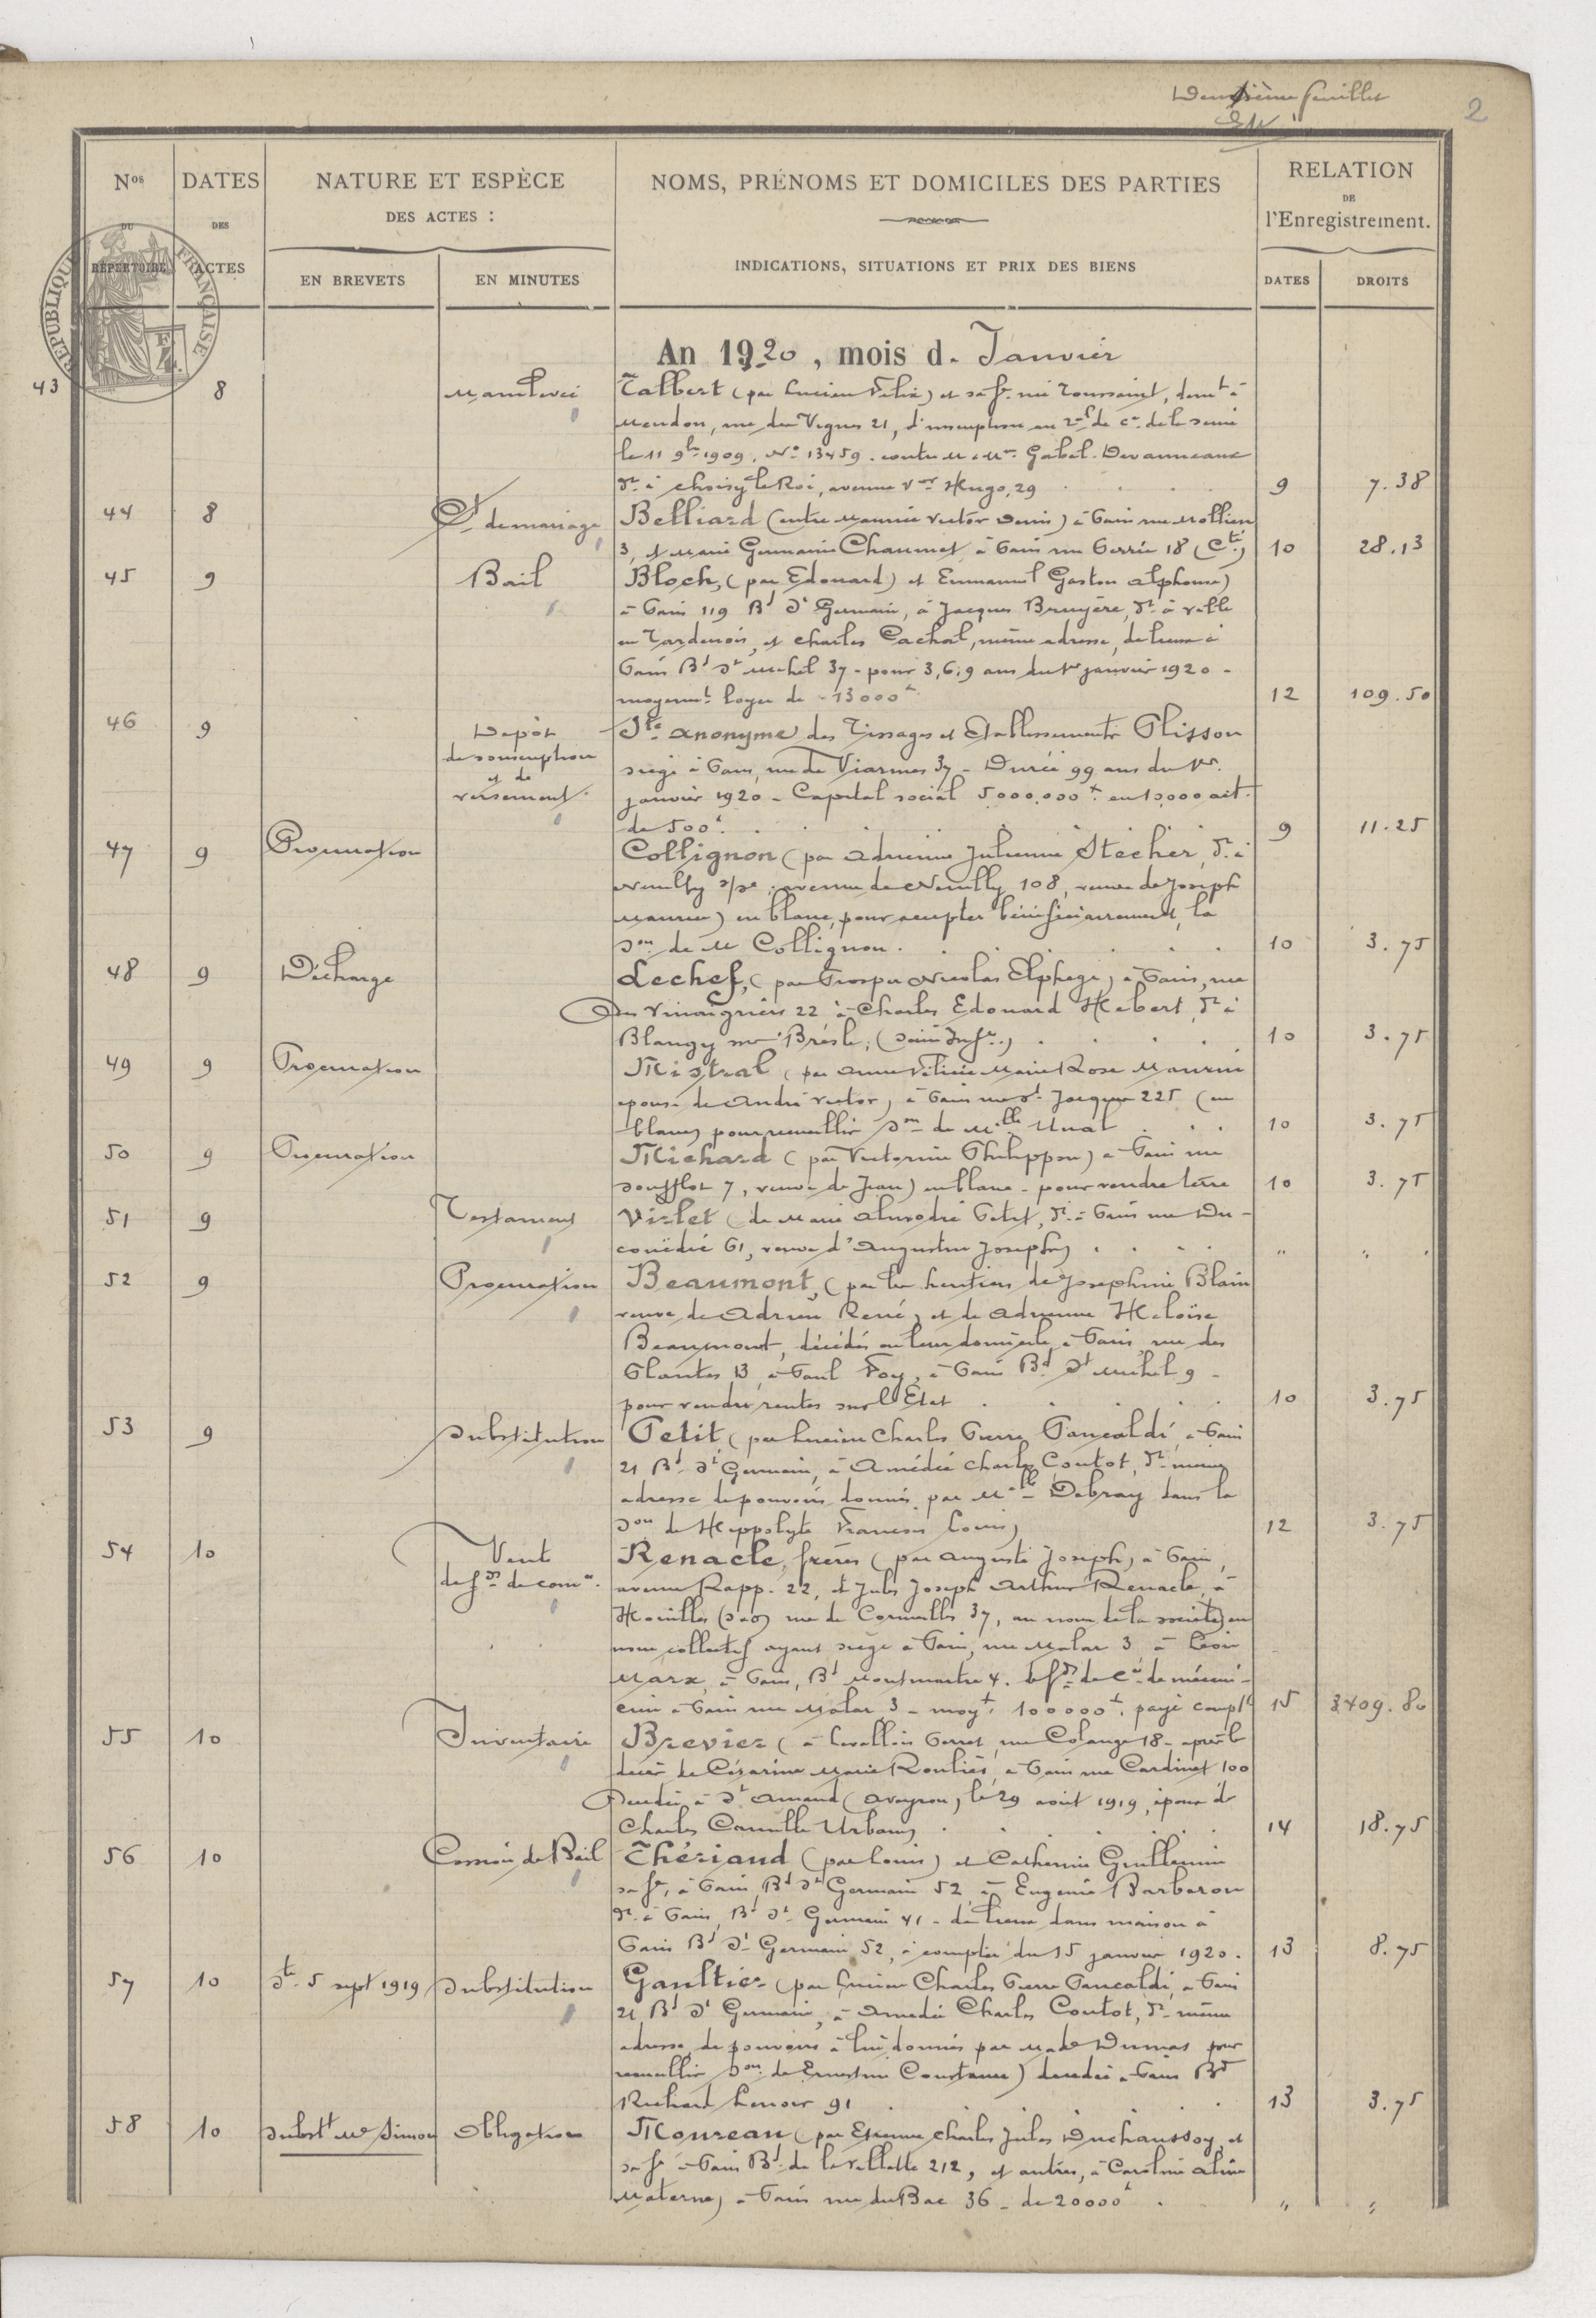
\includegraphics[width=15cm]{repertoire.jpg}
    \caption{Exemple de répertoire de notaire  \textcopyright Archives nationales/DMC, MC/RE/XLIII/42, étude XLIII du notaire Louis Marie Joseph Marotte}
    \label{fig:repertoire}
\end{figure}
\newpage
Les répertoires de notaires ont fait l'objet de vastes campagnes de numérisation, sous la forme de double-page par la société Arkanum\footnote{\cite{bonhomme_defis_2018}, pp. 16} et les images de répertoires de notaires, pour la plupart, sont accessibles en ligne dans la Salle des inventaires virtuelles des AN. \\

La structure régulière des répertoires (structures homogènes en tableaux rendues obligatoires et formalisées par les articles 29 et 30 de la loi du 25 Ventôse an XI) et les exploitations scientifiques potentielles, font de ces documents des candidats idéals pour un projet de reconnaissance. Dès lors, le choix du corpus pour le projet s'est constitué autour d'environ 2000 répertoires de 900 notaires pour la période allant de 1803 à 1944. Chacun de ces répertoires comprenant environ 300 à 500 pages.

\subsection{Le projet Lectaurep : cadre, avancées et objectifs de la phase 3}

Les objectifs du projet Lectaurep sont à terme de proposer\footnote{\cite{chague_lectaurep_2019}} :
\begin{enumerate}
    \item Un outil de recherche intégral pour les publics des archives ;
    \item Des fonctionnalités d'analyses statistiques pour les chercheurs, s'appuyant sur les humanités numériques et les outils du TAL (Traitement automatique du langage) que nous verrons dans la partie \ref{TAL_repertoire} plus en détail ;
    \item Un outil en réseau, mutualisé (\textit{crowdsourcing}) pour les services d'archives, soit la création d'une communauté autour de la transcription. 
\end{enumerate}

Pour répondre à ses besoins, Lectaurep à envisagé la technologie de reconnaissance automatique de structure et d'écriture manuscrite (HTR) ainsi que l'indexation. Enfin, les résultats seront publiés sur une plate-forme dotée d'un moteur de recherche avancée, permettant de requêter directement dans les images de répertoires.\\

Le projet (convention-cadre signée entre INRIA et le Ministère de la Culture en 2016) a connu plusieurs étapes essentielles.

Une première phase (débutée en 2018), à permis de brosser un état de l'art de la reconnaissance automatique et les avantages que celle-ci offre au projet Lectaurep. Ainsi un premier travail de repérage des tableaux\footnote{Pour avoir une idée du repérage des tableaux Cf. Annexes, Figure \ref{fig:tableaux_repertoires}} dans les répertoires de notaires a été mené par Marie-Laurence Bonhomme, alors stagiaire du master TNAH de l'Ecole nationale des chartes. Dans son rapport exploratoire\footnote{\cite{bonhomme_repertoire_2018}}, elle émet les premières préconisations quant au travail de segmentation des tableaux avec le logiciel Transkribus. Cependant, elle constate, toujours dans son rapport, une mauvaise prise en charge des documents de structure tabulaire par le logiciel.\\ 

La phase 2 (2019) du projet a connu plusieurs évolutions, en cause les réorientations dans les choix d'outils, l'acquisition des données et la gestion de projet :
\begin{itemize}
    \item Constitution de jeux de données (images de répertoires de notaires) mis à disposition de l'équipe ALMAnaCH par le DMOASI (Département de la maîtrise d’ouvrage du système d’information) des AN sur la plateforme ShareDocs d'Huma-Num répartis en un \textit{Golden set} et un \textit{Random set} ;
    \item Abandon de l'outil Transkribus et migration vers les outils eScriptorium et Kraken ;
    \item Mise en place d'une plate-forme collaborative basée sur GitLab pour partager les outils nécessaires en appui à la chaîne de traitement Lectaurep (\textit{Pipeline} entre Transkribus et eScriptorium pour le transfert et la compatibilité des données comme le programme Aspyre GT\footnote{CHAGUE, ALix, Aspyre GT, A pipeline to transfer ground truth from Transkribus to eScriptorium, URL : \url{https://gitlab.inria.fr/dh-projects/aspyre-gt}} d'Alix Chagué, ingénieure en humanités numériques à ALMAnaCH pour le projet Lectaurep).
\end{itemize}
\bigskip
L'écosystème de travail pour Letaurep, présenté dans la liste n'a, dans son ensemble, pas été modifié depuis. Les images de répertoires sont réparties en deux sets sur ShareDocs\footnote{Cf. Annexes, Figure \ref{fig:shareDocs}} :
%rajouter image annexes
\begin{enumerate}
    \item Le \textit{Golden set} :  premier set composé d'environ 10000 doubles pages de 41 registres (couvrant la période 1789-1875) numérisés en noir et blanc et en couleur. Il doit servir de base pour créer des documents de vérités terrains ;
    \item Le \textit{Random set} : second set composé 1000 doubles pages aléatoires de quatre campagnes de numérisation récentes en couleur (allant des années 1880 à 1930), doit permettre de tester les modèles de segmentation et de transcription après qu'ils aient été entraînés.
\end{enumerate}
\bigskip
L'abandon de l'outil Transkribus au profit du couple Kraken-eScriptorium, correspond au besoin pour Lectaurep d'avoir la main sur le système d'entraînement des modèles de transcription et de segmentation. En effet, dans Transkribus, les modèles de transcription et les résultats ne sont accessibles que par l’intermédiaire de l'équipe dudit logiciel.
\newpage
Kraken\footnote{Kraken, a turn-key OCR system optimized for historical and non-Latin script material, \textbf{URL de la docummentation} : \url{http://kraken.re/}, \textbf{URL du code source :} \url{https://github.com/mittagessen/kraken}} est le principal logiciel de reconnaissance en ligne de commande (CLI -\textit{Command Line Interface}) utilisé dans le cadre du projet Lectaurep. Il a été développé sur la base du logiciel OCRopus par Benjamin Kiessling. \textit{Open-source}, il permet de binariser les images, de segmenter, et d'entraîner des modèles d'OCR/HTR. Basé sur les réseaux de neurones, il permet d'obtenir de très bons résultats, aussi bien sur les documents imprimés que sur les documents manuscrits dans des caractères latins, hébreux et arabes, avec des taux d'erreur parfois inférieurs à 2\%\footnote{\cite{kiessling_important_nodate}}. Il est également doté d'une API\footnote{\cite{noauthor_kraken_nodate}} (\textit{Application Programming Interface}) qui permet de récupérer le code source pour réutiliser des fonctionnalités spécifiques dans d'autres projets (nous verrons un cas d'application de cette API dans la Partie \ref{partie_3}).\\

eScriptorium\footnote{Cf. Annexes, Figure \ref{fig:appli_eScriptorium}} est l'interface graphique dont s'est doté Kraken dans le cadre du projet Scripta de l'Université PSL\footnote{Scripta PSL, \textit{Scripta PSL | Histoire et pratiques de l’écrit, PSL Scripta}, URL : \url{https://scripta.psl.eu/} (visité le 13/09/2020)}. Il s'agit de la principale interface \textit{web} utilisée par les annotateurs de Lectaurep aux AN, pour réaliser la segmentation et transcrire les images afin de préparer les données d'entraînement (vérités terrains).

La plate-forme eScriptorium est encore en cours de développement. Dès lors, ALMAnaCH est très souvent confronté aux remontées de \textit{bugs} (erreurs d'affichage, mauvais tracés des lignes de segmentation, export de la transcription faussée etc.). L'absence d'un développeur dédié à ALMAnaCH (en cours de recrutement) pour les mises à jour et les corrections de \textit{bugs} sur eScriptorium peut ralentir la chaîne de traitement du côté des AN et l'entraînement des modèles de segmentation ainsi que les tests du côté ALMAnaCH. \\

La phase 3, durant laquelle le stage s'est déroulé, poursuit ces efforts dans l'obtention de meilleures données d'entraînement pour réaliser des modèles de segmentation plus performants. Cela grâce, notamment à des paramétrages différents de Kraken : structuration des transcriptions de vérité terrain à partir des indices de mise en page et de mise en forme, détection des mains d'écriture pour des entraînements de modèles de transcription spécifiques. Les AN poursuivent leur travail d'annotations sur eScriptorium pour obtenir davantage de données d'entraînement. De plus, un certains nombres de fonctionnalités sont en cours de développement pour eScriptorium du côté d'eScripta. ALMAnaCH développe également en interne un certain nombre de fonctionnalités pour Lectaurep hors eScriptorium. L'ensemble de ces fonctionnalités en cours de développement sont résumés dans la Figure \ref{fig:fonctionnalites_eScripto}. Le stage était axé sur le développement de deux de ces fonctionnalités hors eScriptorium à savoir : la génération d'un XML TEI pivot pour les métadonnées (Cf. Partie \ref{partie_2}) et préparer l'évaluation des modèles de transcription (Cf. Partie \ref{partie_3}).\\

De plus afin d'améliorer la visibilité du projet, gagner en confiance et de permettre un retour d'expérience de la part des acteurs de Lectaurep pour servir à d'autres projets similaires, centraliser la documentation et l'histoire du projet, nous avons mis en place un blog \textit{hypothèses} Lectaurep\footnote{Cf. Annexes, Figure \ref{fig:blog_lectaurep}, \textbf{URL du blog} : \url{https://lectaurep.hypotheses.org/}}. Basé sur le CMS \textit{Wordpress} nous avons réalisé un site \textit{web} et préparer l'environnement de rédaction. Des articles sont d'ores et déjà en cours de rédaction.

\begin{figure}[h!]
  \begin{sideways}
    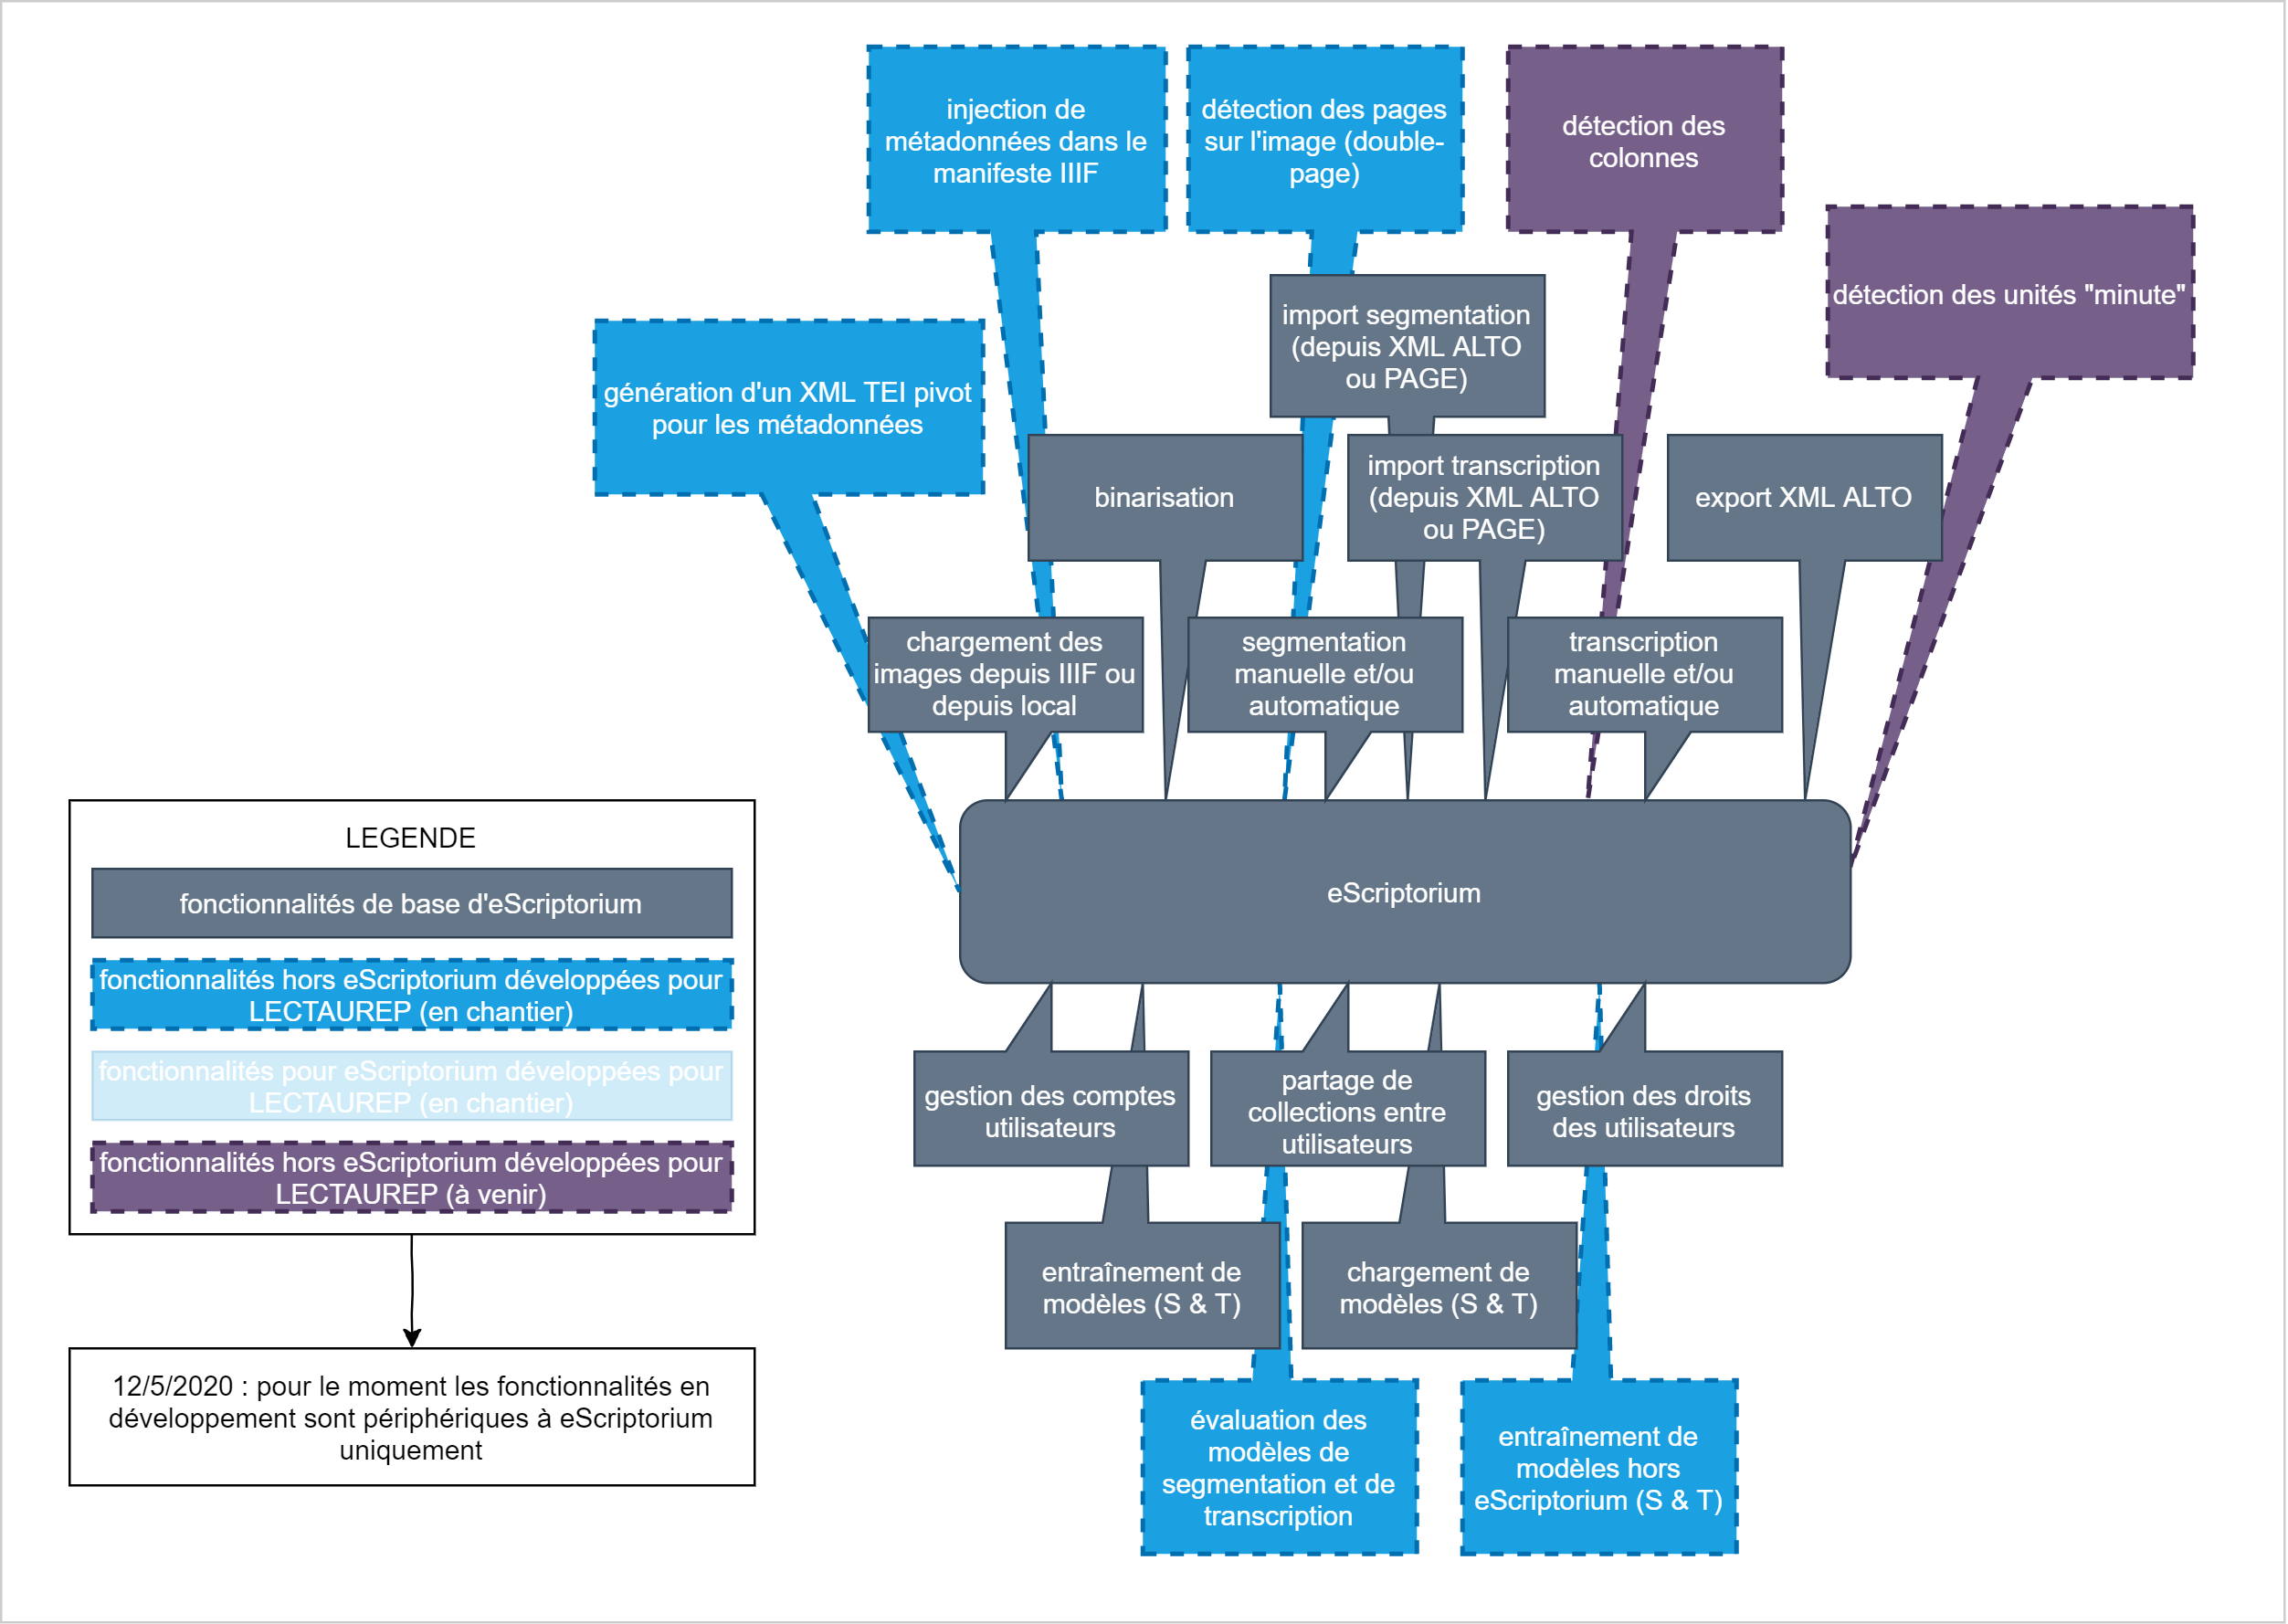
\includegraphics[width=23cm]{schema_fonctionnalites_escriptorium.png}
  \end{sideways}
  \centering
  \caption{Illustration des fonctionnalités en cours de développement durant la phase 3 de Lectaurep \textcopyright A. Chagué, 2020, Diagrams.net}
  \label{fig:fonctionnalites_eScripto}
\end{figure}
\clearpage

\chapter{La reconnaissance automatique des écritures dans Lectaurep : un domaine de l'intelligence artificielle et du traitement automatique du langage naturel (TAL)}

\section{Définir les composantes de l'intelligence artificielle dans le projet}

\subsection{Les champs de l'intelligence artificielle}

En mars 2018, le mathématicien Cédric Villani rend public le rapport, issu d'une mission parlementaire, intitulé \inquote{Donner un sens à l'intelligence artificielle : pour une stratégie nationale et européenne}\footnote{\cite{noauthor_rapport_nodate}}, dans lequel il mène une réflexion détaillée sur l'état de l'art et les atouts de l'intelligence artificielle (IA) en France. Dans ce rapport il apparaît que notre pays compte parmi les quatre premiers au monde, avec la Chine, les États-Unis et le Royaume-Uni pour la production mondiale d'articles sur l'IA et rend compte d'une définition de l'IA non comme :
\begin{quote}
    Un champ de recherches bien défini qu'un programme, fondé autour d'un objectif ambitieux : comprendre comment fonctionne la cognition humaine et la reproduire ; créer des processus cognitifs comparables à ceux de l'être humain.\footnote{\cite{noauthor_rapport_nodate}, pp.9}
\end{quote}
Cette définition n'est peut-être pas la plus complète et la seule qui existe\footnote{\cite{russell_intelligence_2010}, pp.4} mais elle possède l'avantage de définir l'IA comme un champ de recherche en informatique théorique et comme la création de systèmes qui imitent les performances humaines. En 1950, Alan Turing proposait un test hypothétique\footnote{\cite{turing_computing_1950}} afin de savoir si un ordinateur avait acquis l'intelligence opérationnelle d'un humain.\\ 

Le principe était le suivant : après une série de questions posées à l'ordinateur par un humain, le test était réussi si l'humain en question était dans l'incapacité de dire si les réponses provenaient d'un autre humain ou d'un système informatisé. Dès lors, pour passer ce test, et se confondre à l'humain, l'ordinateur devrait posséder les fonctionnalités suivantes : \textbf{le traitement du langage naturel}, pour communiquer, la \textbf{représentation des connaissances}, sous la forme d'une mémoire, un \textbf{raisonnement automatisé}, pour tirer des conclusions logiques de l'expérience mémorisée, et l'\textbf{apprentissage}, pour ajuster ses réponses aux circonstances auxquelles il se retrouve confronté et s'adapter au hasard. Enfin pour simuler entièrement l'humain et passer le test de Turing dit \inquote{complet}, la perception du système pourrait être vérifiée à l'aune de la \textbf{vision artificielle}, pour percevoir les objets, et la \textbf{robotique} pour les manipuler\footnote{\cite{russell_intelligence_2010}, pp. 3}.\\

Parmi les applications de l'IA les plus connues, les véhicules autonomes à l'image de la voiture robotisée de l'université de Stanford en 2005, la reconnaissance de la parole, avec les assistants personnels comme Alexa (2014), les jeux tel que \textit{Deep Blue} d'IBM, le super ordinateur qui a battu le champion mondial Garry Kasparov aux échecs en 1997 suivi par \textit{Alpha Go} en 2015 de Google Deepmind qui bat le champion du monde du jeu de go. On peut également penser aux systèmes de traduction automatique, de type \textit{Google Translate}, qui voit le jour en 2006. Plus récemment la propagation du virus Covid-19, a accentué les usages de l'IA dans les domaines de la santé, notamment pour identifier certains clusters sanitaires localisés avec plus ou moins de succès en se basant sur les données médicales. \\

La plupart de ces applications sont développées dans le cadre d'une \inquote{IA faible}, c'est-à-dire des programmes basés sur des algorithmes\footnote{On définit un \textbf{algorithme} comme une suite d'instructions qui permet d'aboutir à un résultat donné. Une recette de cuisine ou un ensemble de directives pour aller d'un endroit A à un endroit B est un algorithme. En Informatique, il s'agit d'une séquence d'étapes implémentés dans un langage (code) permettant de réaliser un programme ou une tâche précise de ce dernier.} capable de réaliser une tâche précise pour laquelle ils ont été entraînés. On parle alors d'\inquote{IA forte} pour qualifier tout système qui s'affranchirait des volontés humaines et développerait une \inquote{singularité technologique}\footnote{\cite{ganascia_mythe_nodate}}. Cependant ces systèmes pouvant réaliser des tâches en parfaite autonomie, sans contrôle humain, appartiennent encore aux domaines de la science-fiction (lois d'Asimov). D'après ces exemples et le rapport Villani évoqué plus haut, les secteurs prioritaires de l'IA concernent avant tout : la santé, les transports, l'environnement et la défense. \\

Dès lors, comment identifier l'actuelle plus-value de l'IA appliquée à la culture et aux projets patrimoniaux ? Comment le projet Lectaurep illustre-t-il ce mouvement de la culture vers l'IA ? 
La reconnaissance des écritures manuscrites implique de visualiser une image et de détecter le texte (ce qui suppose de disposer de méthodes de perception visuelle), suivre le tracé de l'écriture puis reconnaître les caractères (grâce à des algorithmes de reconnaissance de formes) et enfin reconnaître les mots et les phrases (par le traitement automatique de la langue) pour aller jusqu'à les comprendre (via une modélisation sémantique). Les systèmes de reconnaissance de l'écriture manuscrite utilisés dans Lectaurep, en prenant appuie sur le développement des réseaux de neurones, concernent l'IA et plus précisément le domaine du \textit{deep learning} (DL).\\

\begin{wrapfigure}[13]{r}{5cm}
    \centering
    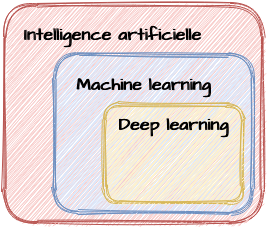
\includegraphics[width=6cm]{champs_IA.png}
    \caption{Les différentes disciplines de l'IA \textcopyright L. Terriel, 2020, Diagrams.net}
    \label{fig:champs_IA}
\end{wrapfigure}
Le DL est une sous discipline du \textit{machine learning} (ML), qui est elle-même une sous-branche de l'IA (Cf Figure \ref{fig:champs_IA}). Le ML et le DL diffèrent dans leur manière dont ils gèrent les données présentée en entrée ainsi que les outils utilisés.\\

Dans un projet ML, le \textit{data scientist} (personne chargée de projets impliquant la gestion de données) choisi des données selon des critères définis (\textit{feature extraction}) à l'avance pour y appliquer des modèles mathématiques de prédiction statistiques (comme le modèle de la régression linéaire, par exemple). Ainsi pour réaliser des prédictions d'achats, des données comme l'âge, le sexe, le revenu, les goûts musicaux, les sports préférés ou autre, pourront être exploitées.\\

La méthode du DL diffère en ce sens qu'il n'y a pas de \textit{feature extraction} réalisé en amont du projet. Dès lors les données présentées en entrée sont dites \inquote{non structurées} : images, textes, sons, etc. En utilisant des algorithmes de réseaux de neurones profonds, on charge le programme d'extraire par lui-même les caractéristiques des données d'exemple en entrée et d'émettre des prédictions à partir de modèles statistiques et mathématiques, empruntés au ML. Ainsi, dans un projet DL de reconnaissance de formes basé sur des images, le programme sera dans la capacité de relever des amas de pixels caractéristiques et redondants correspondants à une forme en particulier. Cependant nous verrons que dans le cas d'un apprentissage semi-supervisé, comme dans Lectaurep, certains types de données peuvent être étiquetés comme par exemple les zones contenant du texte sur les différents tableaux du répertoire, sont représentées sous la forme de coordonnées de polygones et de lignes de textes. Cela permet d'améliorer les prédictions de transcription grâce à un modèle entraîné par des réseaux de neurones.\\ 

Nous allons par la suite, appréhender les différentes étapes à initier lors d'un projet de reconnaissance d'écritures manuscrites tel que Lectaurep. Cela s'apparente aux traitements classiques du \textit{deep learning}, à savoir la préparation des données, l'entraînement des modèles, et enfin prédiction la machine automatique.

\subsection{L'étape de préparation et d'acquisition des données d'apprentissage de Lectaurep}

A l'ère du \textit{Big Data}, les données sont partout et constituent la base des projets DL. Par exemple un modèle devant reconnaître des motos et des voitures dans des images, devra disposer d'un grand nombre d'exemples assez variés pour, à terme, être capable d'opérer les bonnes distinctions dans un corpus d'images représentant plusieurs moyens de transports différents. Encore faut-il que ces données, pour permettre une classification correcte, soient de bonne qualité. Dans le projet Lectaurep, ces données sont les images de répertoires de notaires. Ce sont elles qui vont servir de données d'entraînement au modèle. Cependant, à la différence des écritures imprimées, généralement lisibles par une machine, les écritures manuscrites constituent un problème d'un autre ordre : \\
\begin{quote}
    Certaines écritures restent difficiles à déchiffrer [...] comme les écritures d'archives et historiques, car à la complexité d'une écriture que seuls les paléographes peuvent déchiffrer, s'ajoute la compréhension d'une langue qui n'est plus parlée ou qui a évoluée. Pourtant toutes ces écritures ont été produites par des hommes avec l'objectif de se faire comprendre sans erreur par d'autres hommes.\footnote{\cite{kermorvant_reconnaissance_2019}}
\end{quote}
\newpage
Les écritures du $ XIX^{e}$ siècle contenues dans les répertoires de notaires constituent un réel défi pour la lecture machine. On constate de grandes variabilités de formes d'écriture d'un scribe à un autre. Aux aspects graphologiques liés à la pression de la plume, à l'inclinaison des traits des lettres, à l'alignement des mots par rapport aux lignes de bases, ainsi qu'à la formes des lettres qui varient d'un clerc à un autre, s'ajoutent également la spécificité des outils utilisés suivant le contexte d'écriture. Pour la calligraphie, le clerc préférera la plume d'oie, tandis que pour écrire plus vite ou pour \inquote{expédier} il choisira la plume en métal sous la dictée du notaire. Cela induit le fait que, parfois dans un même répertoire de notaire par des formes de polices d'écritures très différentes peuvent se côtoyer : ronde, gothique, minuscule caroline, italique ou cursive anglaise, lettres capitales etc. Les écritures des répertoires sont rarement uniformes. (Cf. Figure \ref{fig:ecritures_XIX}).
\begin{figure}[!h]
    \begin{minipage}[c]{.46\linewidth} 
        \centering
        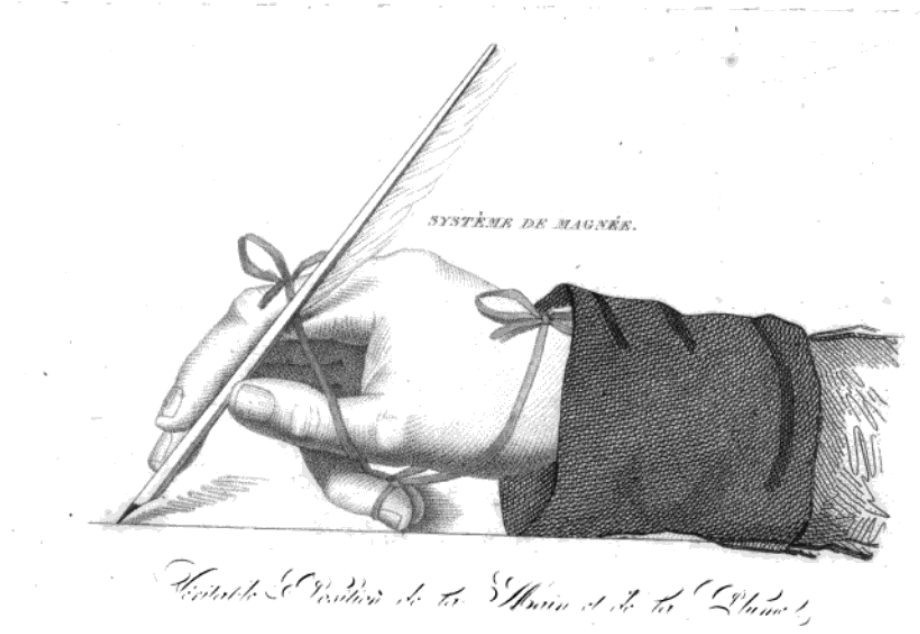
\includegraphics[width=7cm]{ecritures_XIX/ecriture_magnee.png}
    \end{minipage}
    \hfill%
    \begin{minipage}[c]{.46\linewidth}
        \centering
        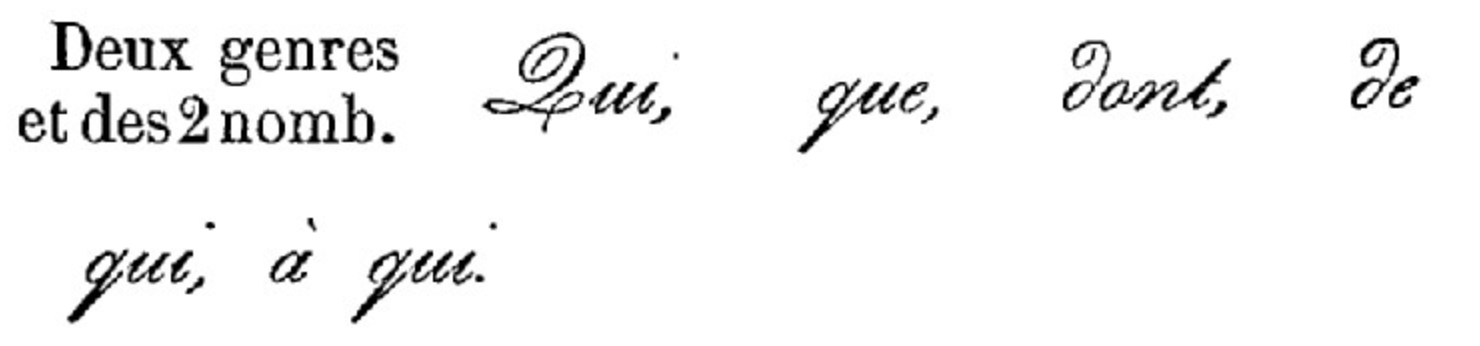
\includegraphics[width=10cm]{ecritures_XIX/exemple_Q_d.png}    
    \end{minipage}
\end{figure}
\begin{figure}[!h]
        \centering
        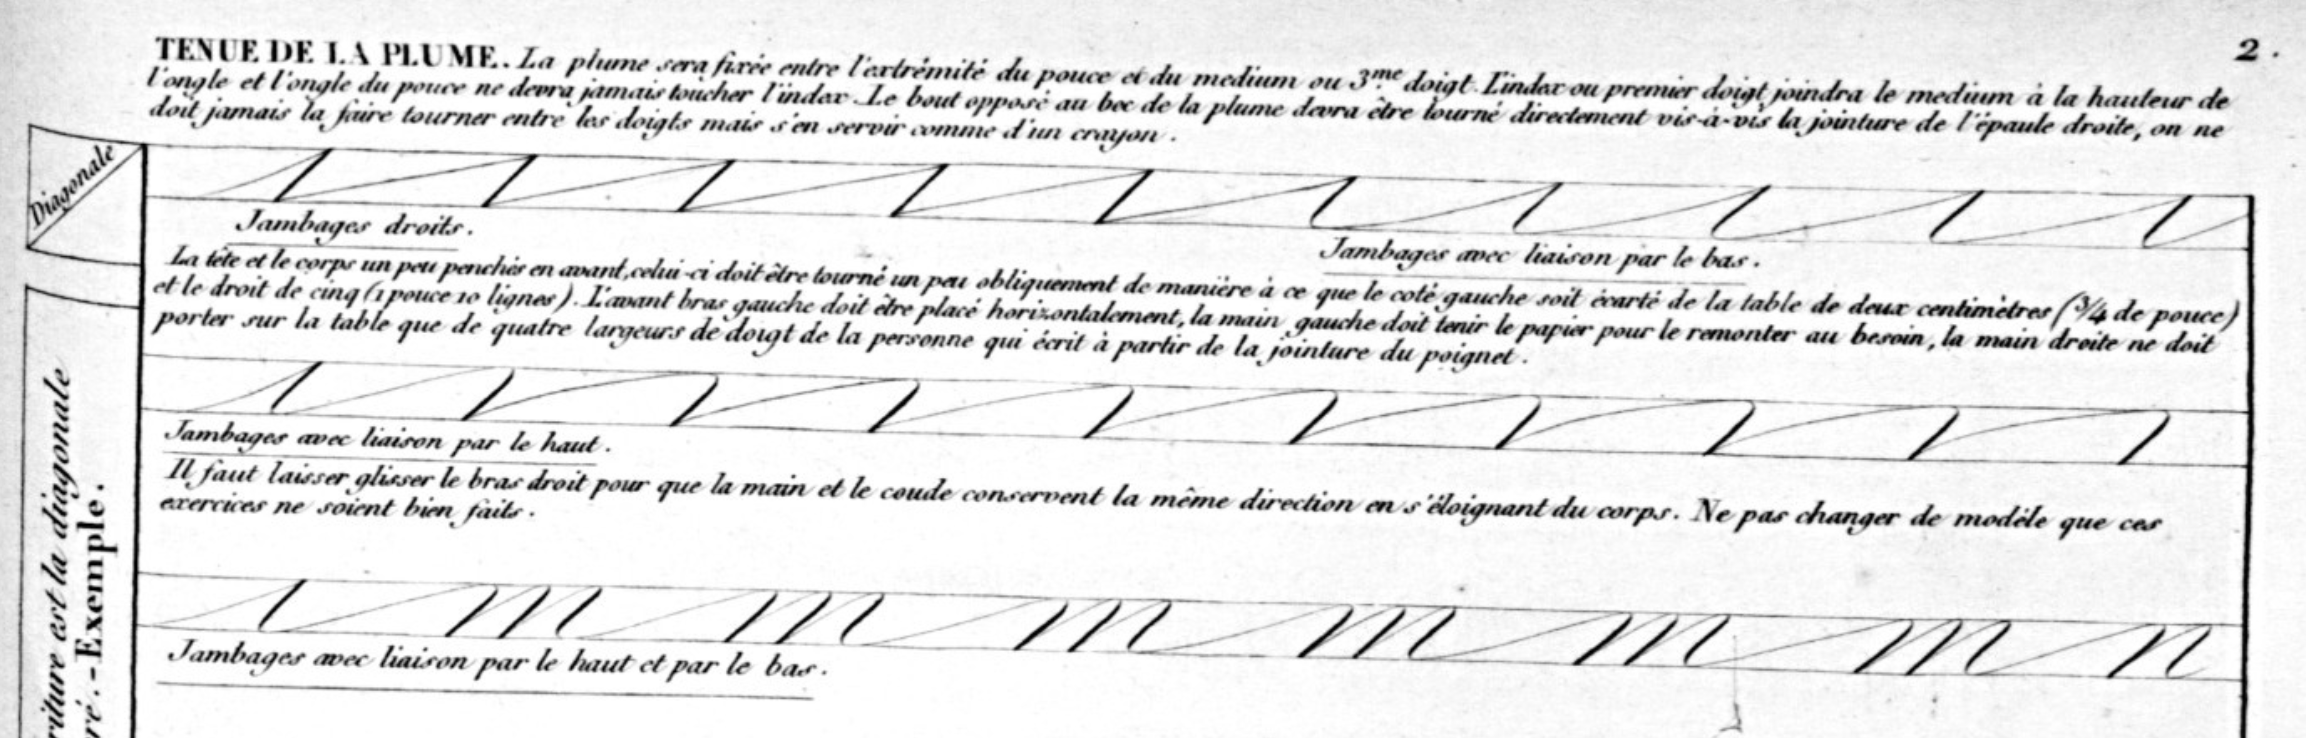
\includegraphics[width=12cm,height=9cm]{ecritures_XIX/hampes_jambages.png}
\end{figure}
\begin{figure}[!h]
    \begin{minipage}[c]{.46\linewidth} 
        \centering
        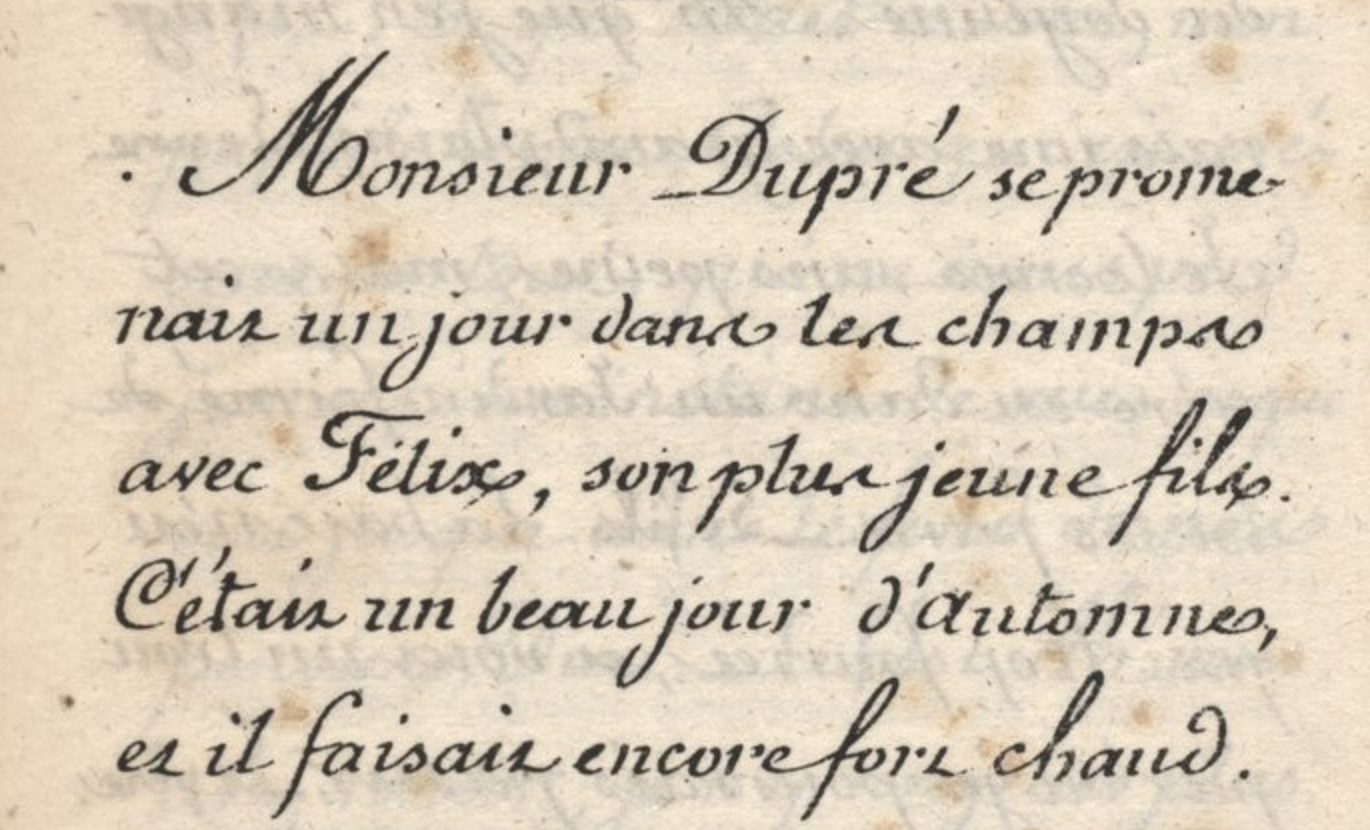
\includegraphics[width=8cm,height=7cm]{ecritures_XIX/ecriture_fin_anc_regime.png}
        \end{minipage}
    \hfill%
    \begin{minipage}[c]{.46\linewidth}
        \centering
        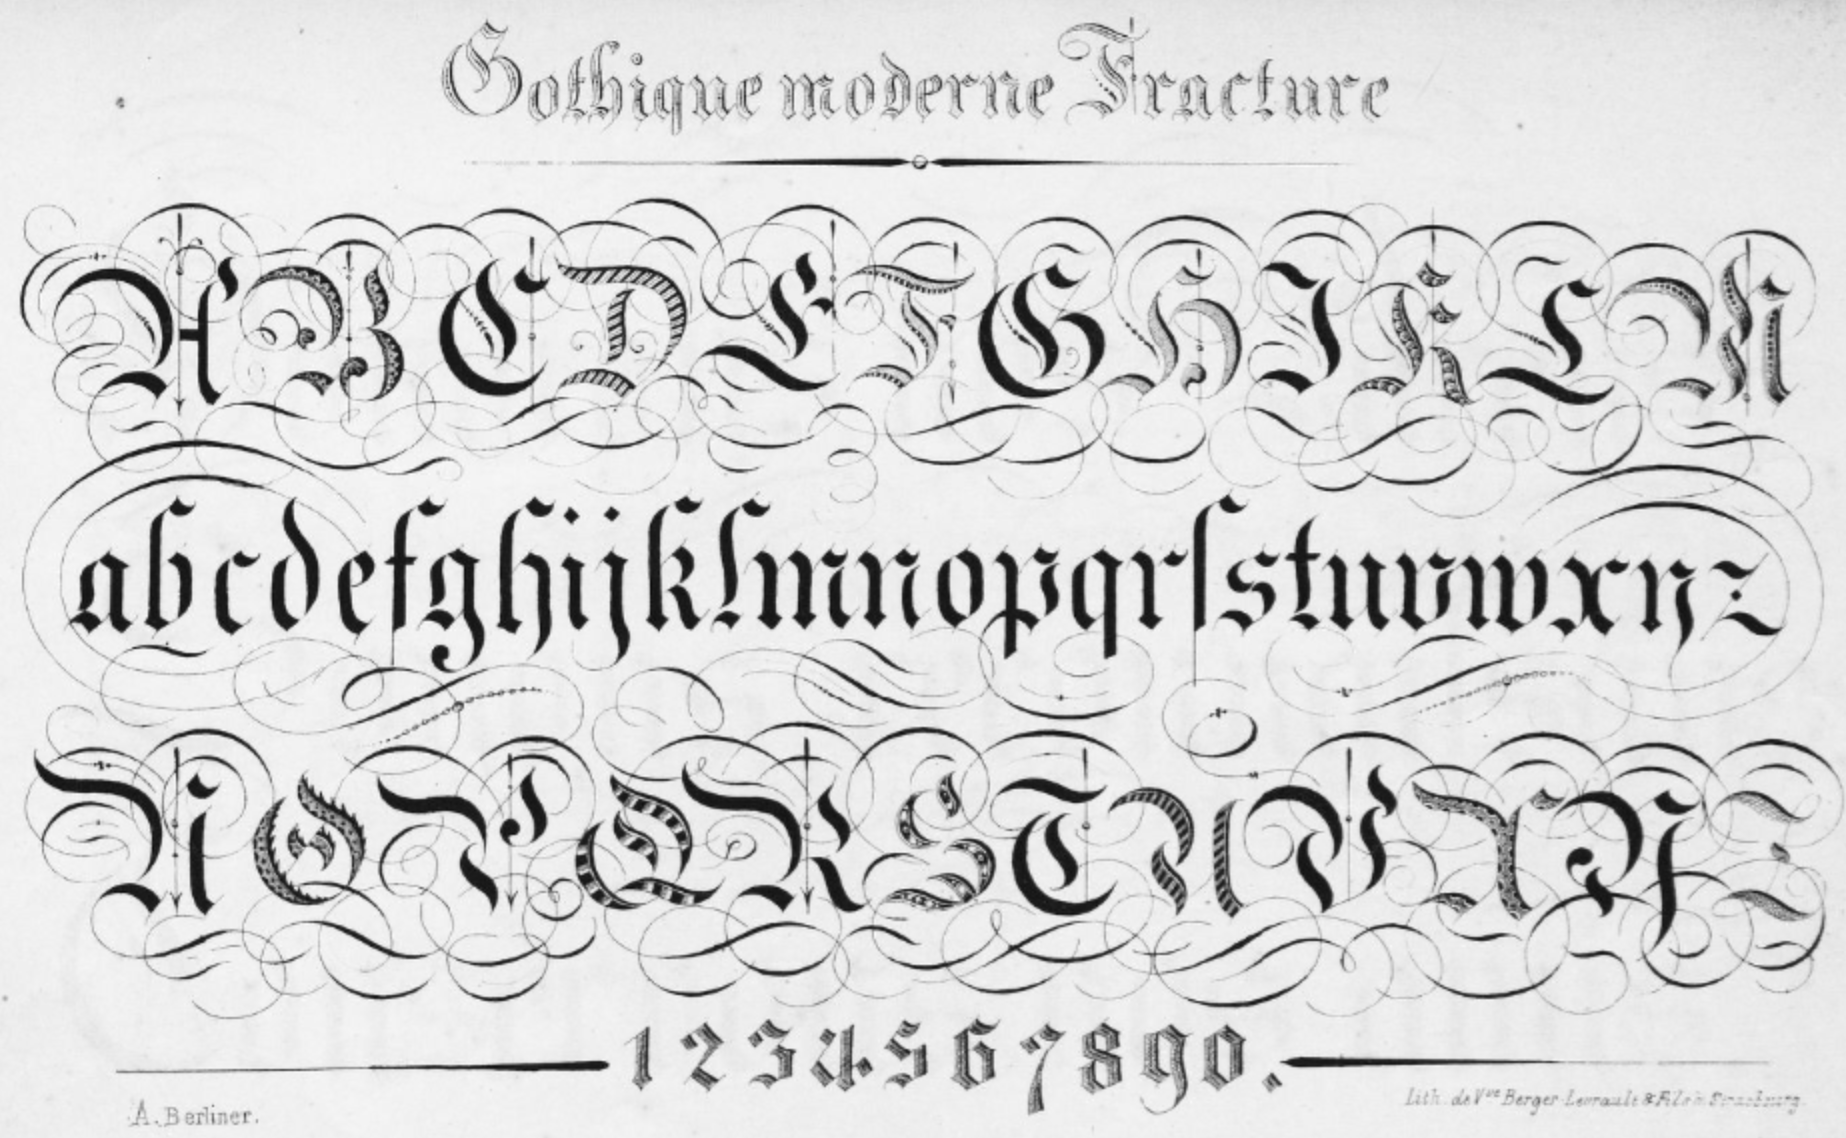
\includegraphics[width=8cm,height=7cm]{ecritures_XIX/gothique_moderne_fraktur_berliner.png}
    \end{minipage}
\end{figure}
\begin{figure}[!h]
        \centering
        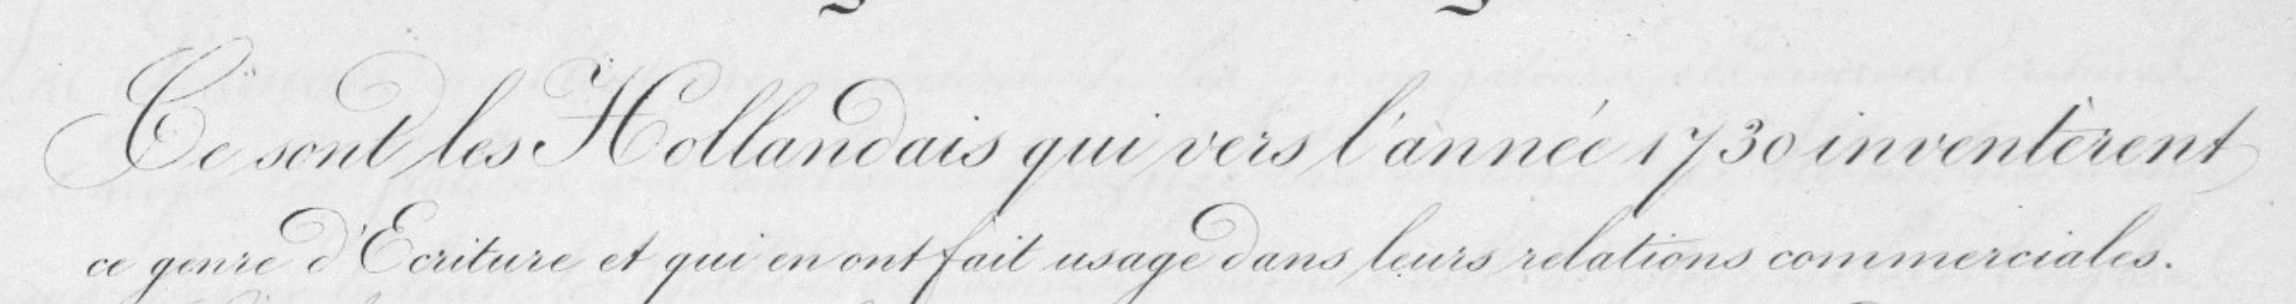
\includegraphics[width=18cm]{ecritures_XIX/cursive_anglaise_berliner.png}
\end{figure}
\begin{figure}[h!]
    \centering
    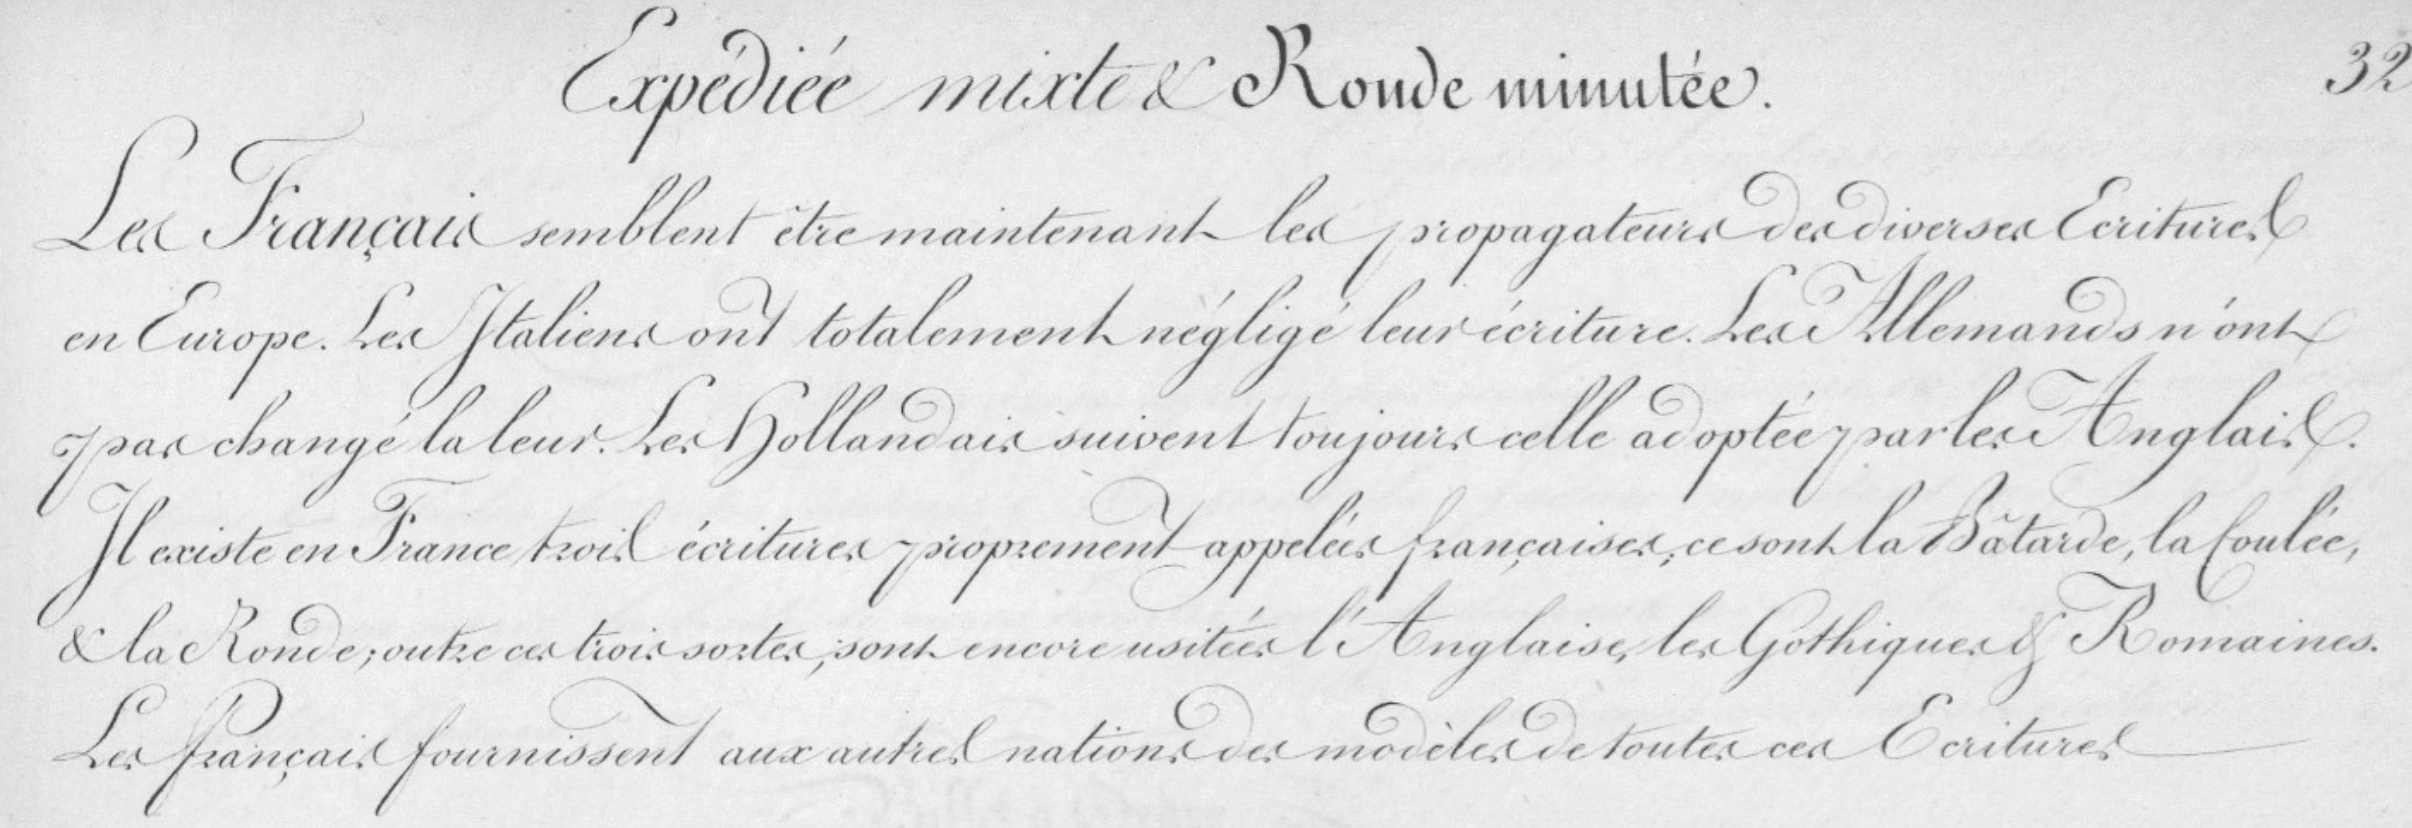
\includegraphics[width=13cm,height=9cm]{ecritures_XIX/ronde_minutee_berliner.png}    
    \label{fig:my_label}
\end{figure}
\begin{figure}[!h]
        \centering
        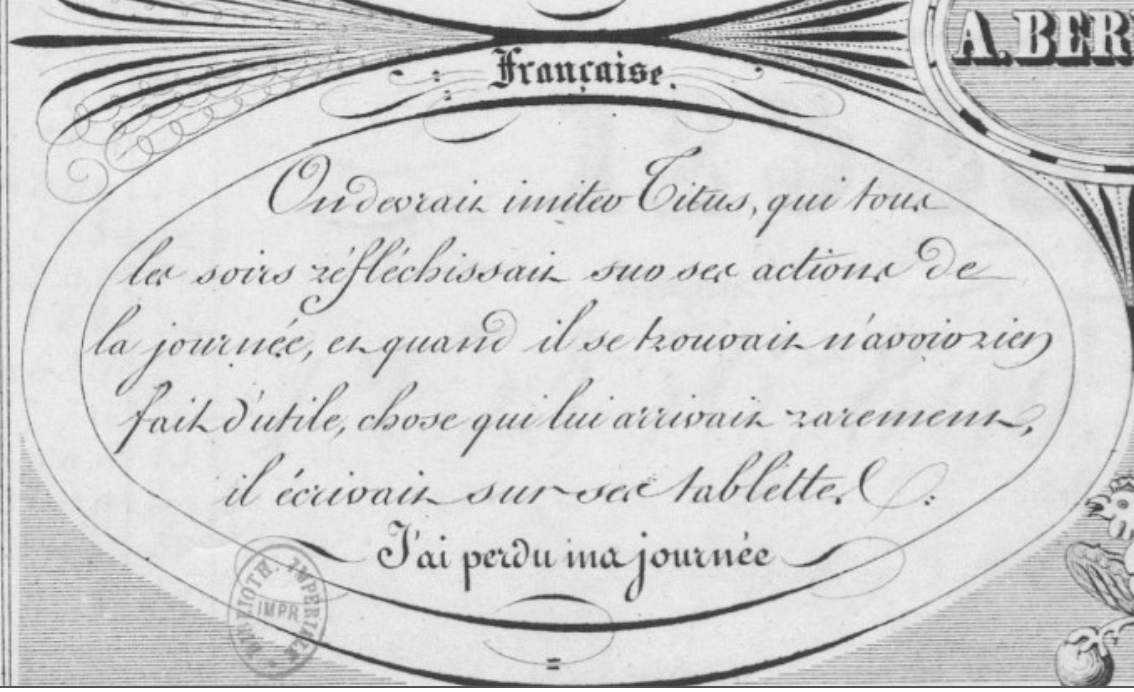
\includegraphics[width=10cm,height=6.5cm]{ecritures_XIX/ecriture_latine_berliner.png}
\end{figure}
\begin{figure}[!h]
        \centering
        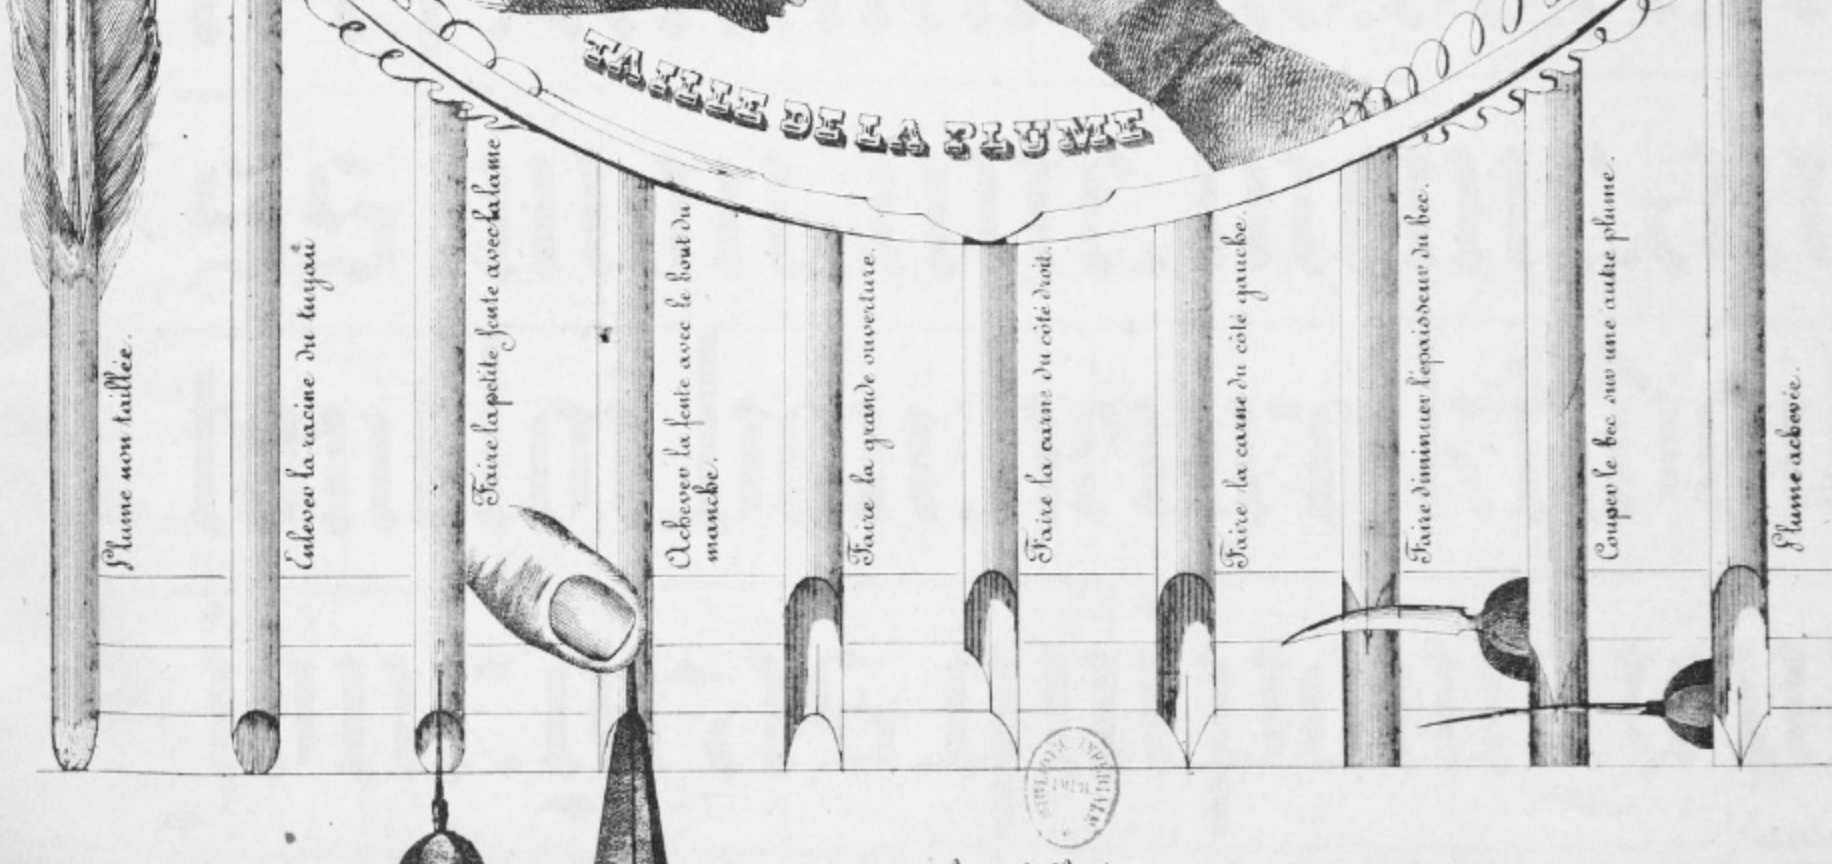
\includegraphics[width=10.5cm,height=8cm]{ecritures_XIX/taille_plume_berliner.png}
        \caption{\textbf{Exemples de types d'écritures $ XIX^{e}$ siècle rencontrées dans les répertoires de notaires}, de gauche à droite et de haut en bas : système d'écriture dit \inquote{de Magnée} extrait de \cite{magnee_parfait_1828}, exemple de \inquote{d} delta et de \inquote{Q} majuscule archaïque repris de \cite{molliard_methode_1861}, exemples de modules de tracés des jambages et des hampes \cite{werdet_innovation_1841}, d'écriture \inquote{coulée} Ancien Régime repris de \cite{fremont_cahiers_1837}, exemples de gothique moderne dite \inquote{fracture}, de cursive anglaise, de ronde minutée, d'écriture latine et de taille de plume extraits de \cite{berliner_cours_1862}.}
    \label{fig:ecritures_XIX}
\end{figure}
\clearpage
En plus de ces écritures très différentes, les images de répertoires n'ont pas été numérisées avec la même qualité : on retrouve parfois du noir et blanc ou des cadrages non-homogènes\footnote{Pour consulter des exemples de différentes qualités numérisation, Cf. Annexes \citecode{/C-Application\_Kraken\_Benchmark/sets\_test/sets\_tests\_lectaurep/}}. Dès lors ces images, avant de servir d'exemples d'entraînement, peuvent subir des \textbf{pré-traitements} comme la binarisation (passage au noir \& blanc), la découpe des doubles pages des images de répertoires pour fournir un tableau au système, et un recadrage.\\

Une fois ces pré-traitements images effectués, on réalise généralement une extraction des caractéristiques (\textit{features}) de l'image. On identifie les différentes zones de texte, paragraphes, lignes et parfois lettres dans une phase. On réalise une opération de \textbf{segmentation}. Dans un premier temps et durant sa phase 1, Lectaurep utilisé l'outil Transkribus pour passer ensuite à l'usage du segmenteur de Kraken inclus dans la plate-forme eScriptorium afin d'effectuer une segmentation des zones des tableaux repérés par Marie-Laurence Bonhomme dans le répertoires \footnote{Cf. Figure \ref{fig:tableaux_repertoires}, consulter également \cite{bonhomme_defis_2018}, pp. 20-26.}. Ces zones correspondent à la ligne de base du texte (\textit{baseline}) et à des ensemble de points entourant du texte (\textit{polygons}) et constituent des coordonnées. Ces zones sont généralement observables dans des exports en XML ALTO ou XML PAGE (pour plus de précisions sur ces formats consulter la Partie \ref{partie_2}). Si cette segmentation peut s'effectuer à la main dans eScriptorium ces zones constituent en elles-mêmes des données d'entraînement pour créent des modèles de segmentation, qui permettent de relever ces zones de manière automatique et ainsi gagner du temps. \\

Après cette phase de segmentation, vient celle de la \textbf{transcription manuelle} contrôlée. Elle est réalisée par les annotateurs des AN du projet Lectaurep et doit servir de \textbf{vérité terrain} (\textit{ground truth}) afin d'entraîner et de paramétrer le moteur HTR disponible dans le CLI Kraken (hors eScriptorium actuellement). Ces données de vérité terrain seront comparées avec les prédictions effectuées par le système HTR pour évaluer le taux d'erreur par transcription. Cependant, la transcription \inquote{à la main} (dans eScriptorium) demandent d'effectuer un certains nombres de normalisation et impose des règles de transcription. Ainsi, cela évite de donner aux systèmes deux interprétations d'un même caractère. \\

En effet, comment retranscrire avec le clavier des ligatures (fusion de deux ou trois graphèmes pour en former un nouveau), un \inquote{s} final en forme archaïque et moderne, un \inquote{s} long, un \inquote{d} en forme de delta recourbé ou en hampe archaïque, faut-il rajouter des majuscules aux noms propres lorsqu'elles sont absentes ? 
\newpage
\begin{figure}[H]
    \begin{minipage}[c]{.46\linewidth} 
        \centering
        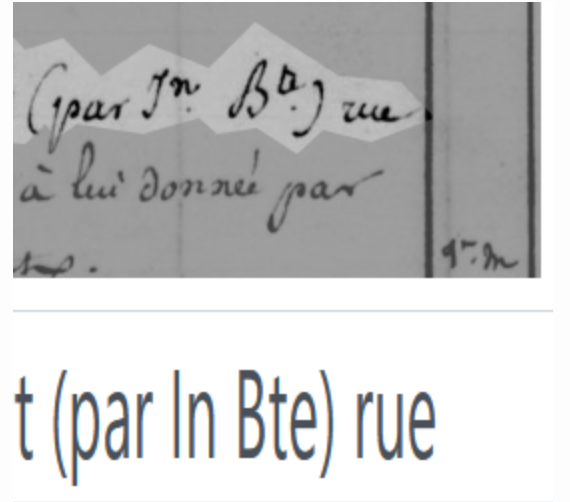
\includegraphics[width=8cm,height=7cm]{cas_abbr_char_eScriptorium/cas_1.png}
        \end{minipage}
    \hfill%
    \begin{minipage}[c]{.46\linewidth}
        \centering
        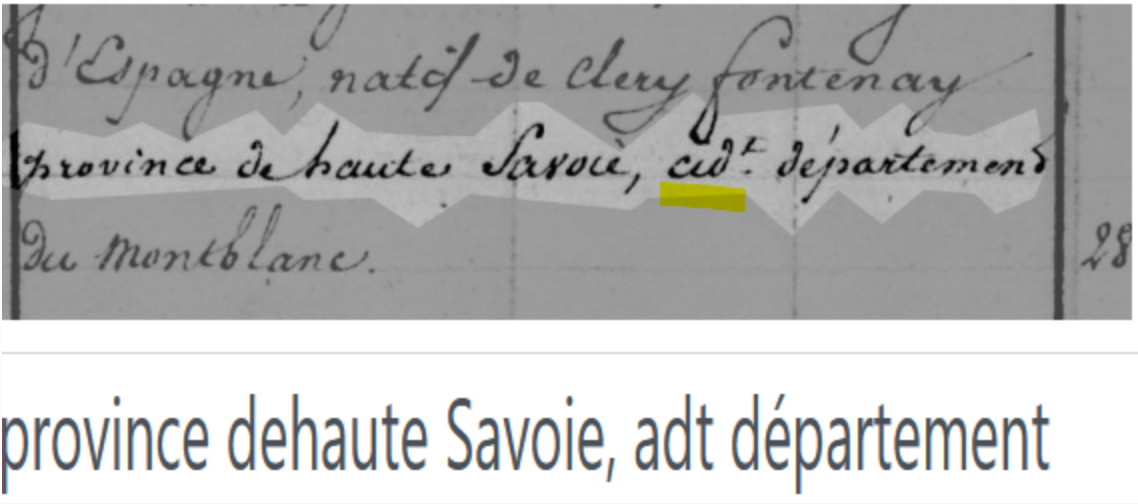
\includegraphics[width=8cm,height=7cm]{cas_abbr_char_eScriptorium/cas_3.png}
    \end{minipage}
    \hfill%
    \begin{minipage}[c]{.46\linewidth}
        \centering
        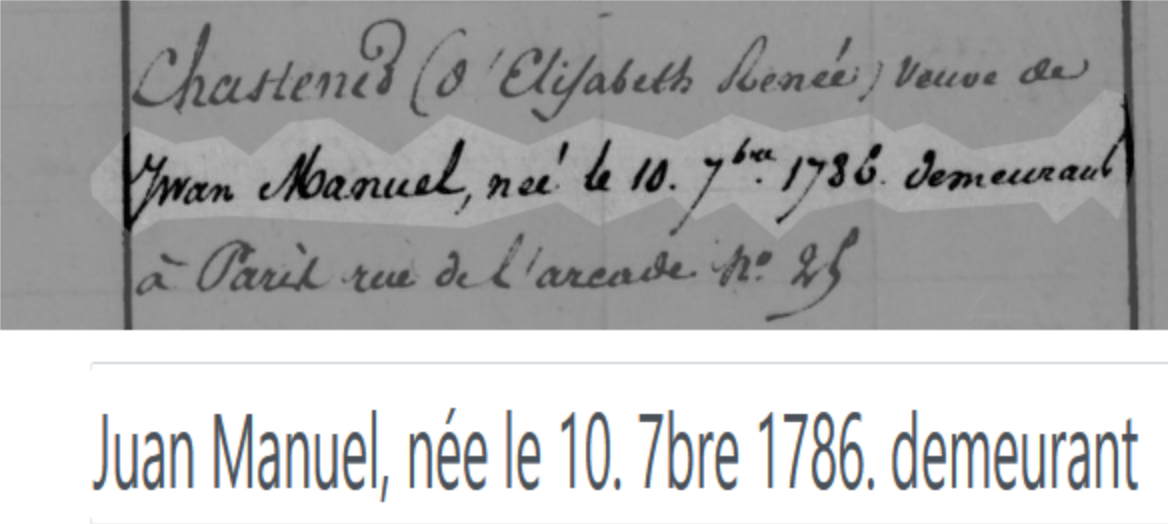
\includegraphics[width=8cm,height=7cm]{cas_abbr_char_eScriptorium/cas_4.png}
    \end{minipage}
    \hfill%
    \begin{minipage}[c]{.46\linewidth}
        \centering
        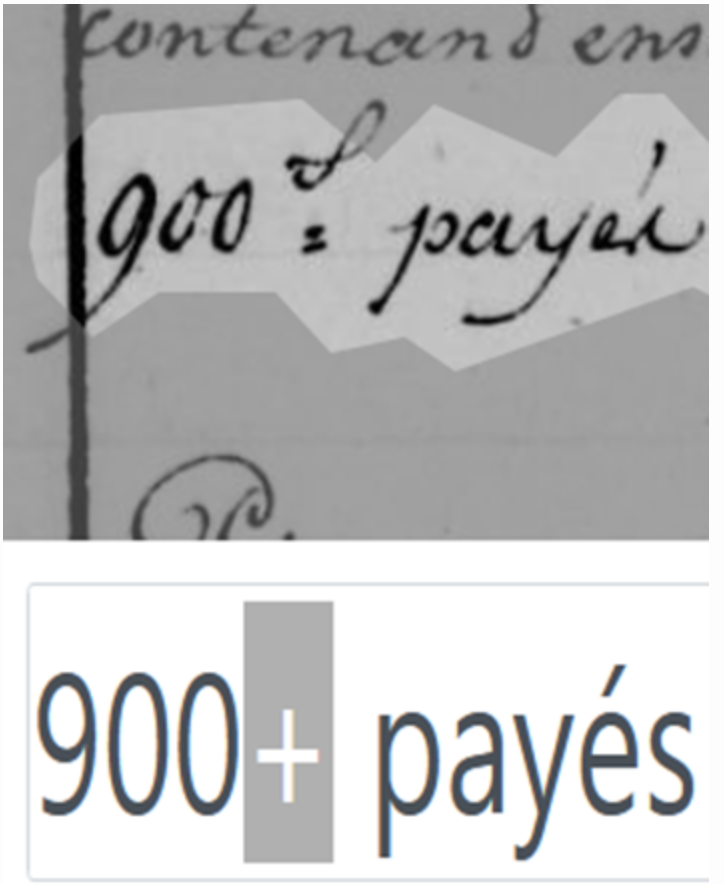
\includegraphics[width=8cm,height=7cm]{cas_abbr_char_eScriptorium/cas_5.png}
    \end{minipage}
    \hfill%
    \begin{minipage}[c]{.46\linewidth}
        \centering
        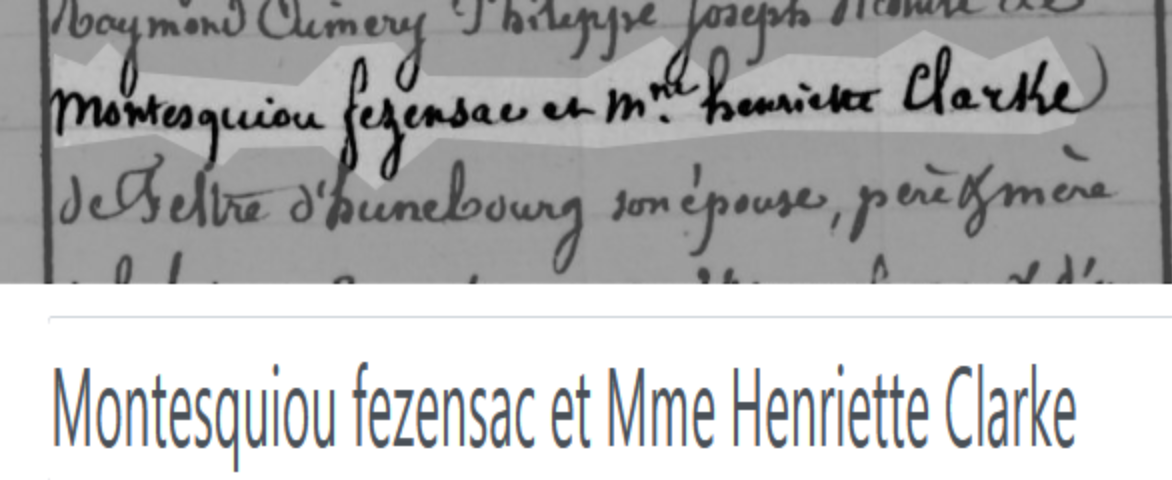
\includegraphics[width=8cm,height=7cm]{cas_abbr_char_eScriptorium/cas_8.png}
    \end{minipage}
    \hfill%
    \begin{minipage}[c]{.46\linewidth}
        \centering
        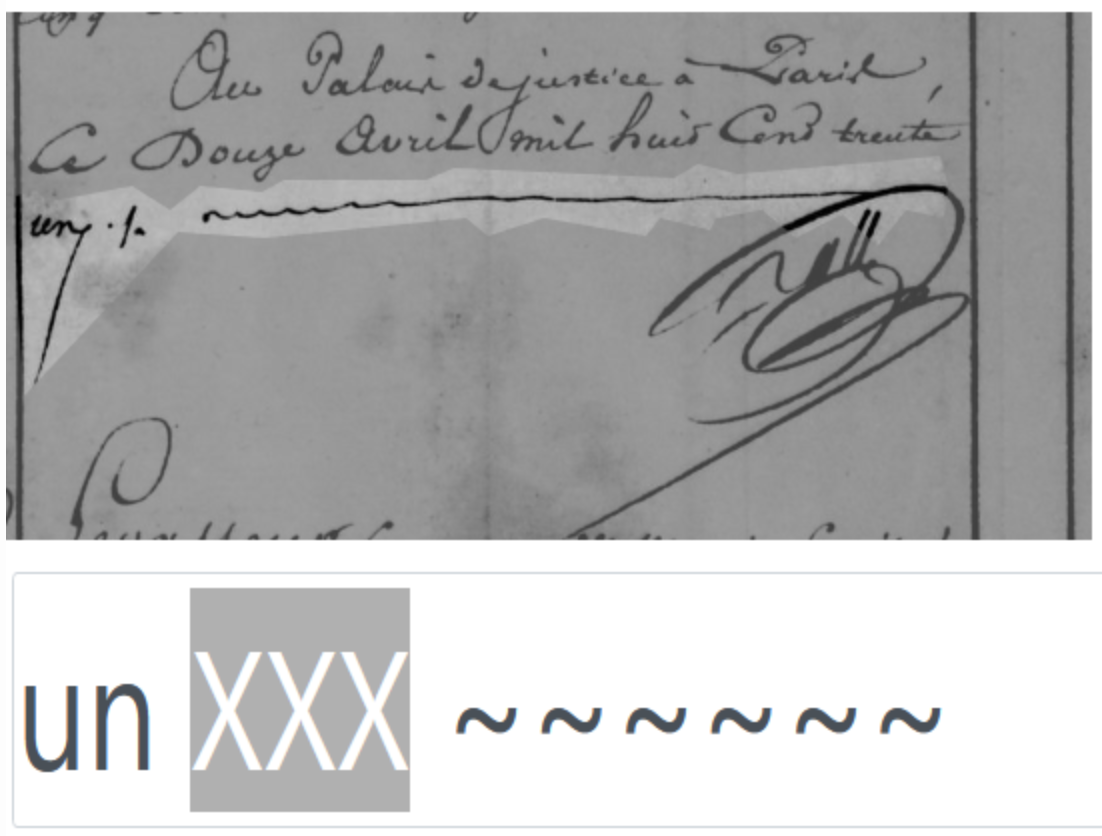
\includegraphics[width=8cm,height=7cm]{cas_abbr_char_eScriptorium/cas_9.png}
    \end{minipage}
        \caption{Quelques exemples de transcriptions réalisées par des annotateurs de Lectaurep dans eScriptorium. \textcopyright Captures fournies par A. Rostaing (AN/DMC), 2020, eScriptorium}
    \label{fig:exemples_eScriptorium}
\end{figure}
\newpage
Ces questionnement ne sont pas encore formalisées par le DMC des AN qui effectue actuellement un travail pour formaliser des règles. Cela reste encore une tâche difficile à réaliser dont les cas particuliers sont nombreux (pour visualiser les segments, choix de transcription et quelques règles de normalisation des abréviations et caractères spéciaux appliqués par les annotateurs de Lectaurep sur eScriptorium Cf. Figure \ref{fig:exemples_eScriptorium}).\\

Les étapes de préparation des données sont donc essentielles car elles déterminent les résultats, certaines erreurs pouvant constituer des \textbf{biais de prédictions} qui fausse ces derniers. Une fois les données acquises il est possible de passer à l'apprentissage pour la création de modèles. 

\subsection{L'étape d'apprentissage et d'entraînement des modèles}

On distingue généralement trois types d'apprentissage machine : 
\begin{itemize}
    \item \textbf{l'apprentissage supervisé} : les données sont catégorisées par des étiquettes \textit{features} selon des caractéristiques en entrée de l'algorithme. C'est une étape de préparation lourde en ressources humaines car il est \inquote{guidé} par l'homme. L'algorithme se charge alors d'ajuster ces marges d'erreurs au fil des itérations durant l'entraînement, jusqu'à créer un modèle généralisable à des données, cette fois, non étiquetées, et qui obtiennent de bons résultats. Par exemple, dans le cadre d'une application de détection de spam, les caractéristiques en entrée du système pourraient être l'objet, l'expéditeur, le message lui-même et les étiquettes \inquote{spam} ou \inquote{non-spam} ;\\
    \item \textbf{l'apprentissage non-supervisé} : les données en entrée ne sont pas catégorisées, c'est donc à l'algorithme lui-même de détecter des similarités entre ces dernières. Il s'applique généralement à des jeux de données de très grande taille et non homogènes où l'utilisation d'humains dans la préparation des données pourrait s'avérer fastidieuse ;\\
    \item \textbf{l'apprentissage mixte ou semi-supervisé} : ce type d'apprentissage tente de réaliser un compromis entre les deux types d'apprentissage présenté ci-dessus. L'algorithme est guidé au minimum avec un petit nombre d'étiquettes et se charge ensuite de classifier et de regrouper les autres caractéristiques de manière autonome.\\
\end{itemize}

Dans le cadre de Lectaurep, il s'agit plutôt d'apprentissage semi-supervisé qui montre de bonnes performances dans l'entraînement de modèle HTR. Le moteur HTR de kraken, basé sur des réseaux de neurones, est guidé par la segmentation des zones et lignes de textes sur l'image sous la forme de coordonnées, et se charge ensuite d'effectuer la prédiction des formes de caractères. Nous verrons plus par la suite les types de réseaux de neurones qui permettent de réaliser ce type d'apprentissage.

\subsection{La prédiction par la machine}

Il s'agit de l'étape ultime qui consiste à vérifier la capacité du modèle à traiter correctement l'information. Lors de la phase d'apprentissage, le modèle tire des conclusions de ses calculs statistiques. Dans le cadre de l'évaluation du modèle HTR, il doit se rapprocher au maximum de la transcription vérité terrain réalisée manuellement en amont, sous la supervision d'humains. Lors de l'apprentissage, il est généralement recommandé de toujours découper son set d'apprentissage en deux (Kraken, configure par défaut un découpage en deux parties égales, mais il est possible de le paramétrer) :

\begin{itemize}
    \item un set de données d'entraînement (\textit{training set}) ;
    \item un set de données de test (\textit{test set}).\\ 
\end{itemize}

Un aspect à prendre en compte dans ces cas d'apprentissage concerne le \textbf{sur-entraînement} (\textit{overfitting}). Le modèle a été entraîné avec des données homogènes (ensemble du set d'apprentissage), si bien, qu'il devient trop étroitement lié à ces dernières. Il est alors incapable de se généraliser à d'autres données. 

Le cas inverse correspond au \textbf{sous-entraînement} (\textit{underfitting}), c'est-à-dire que l'on a fourni trop peu de données pour le modèle qui est, non seulement incapable de faire des prédictions sur les données avec lesquelles il a appris (\textit{training set}), mais qui ne peut pas non plus se généraliser à de nouvelles données. Nous reverrons ces cas lors de la réalisation de tests de qualité de transcription présentés en partie \ref{partie_3}.\\ 

Lors de l'apprentissage les réseaux de neurones présents dans Kraken passent par plusieurs états (\textit{epochs}), sont observables lors de son utilisation (Cf. Figure \ref{fig:epoque_kraken_prompt}) \\

\begin{figure}[h]
    \centering
    \centerline{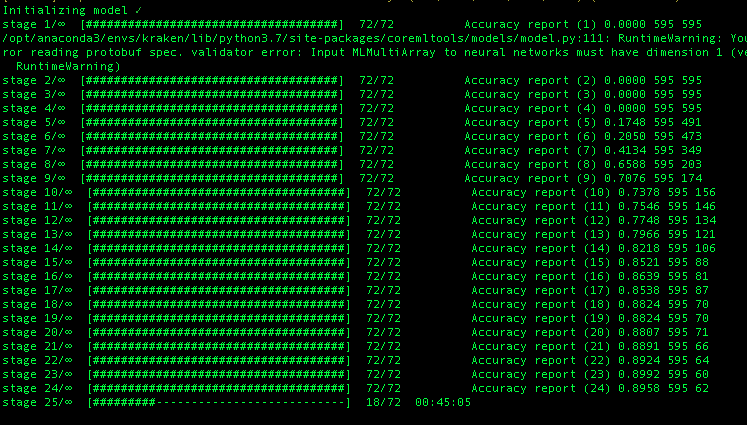
\includegraphics[width=12cm]{exemples_epoques_kraken.png}}
    \caption{Illustration des époques (\textit{stage}) d'apprentissage pour la création d'un modèle de transcription avec Kraken \textcopyright L. Terriel, 2020, Kraken/cluster de calcul INRIA-RIOC}
    \label{fig:epoque_kraken_prompt}
\end{figure}
\newpage
A chacune de ces itérations ou époque d'apprentissage, Kraken produit un modèle (format .mlmodel) et l'évalue à l'aide de métriques (\textit{accuracy report}) qui s'appuient sur la précision (\textit{precision})\footnote{la \textbf{précision} (\textit{precision}) ou valeur prédictive positive, est une mesure permettant d'estimer la proportion des items pertinents parmi l'ensemble des items proposés.
$$ \text{precision}_i = \frac{nb\,de\,documents\,correctement\,attribues\,a\,la\,classe}{nb\,de\,documents\,attribues\,a\,la\,classe} $$}, le rappel (\textit{recall})\footnote{le \textbf{rappel} (\textit{recall}) ou sensibilité est la proportion des items pertinents proposés parmi l'ensemble des items pertinents. 
$$ \text{rappel}_i = \frac{nb\,de\,documents\,correctement\,attribues\,a\,la\,classe}{nb\,de\,documents\,appartenant\,a\,la\,classe} $$}, le F1 score\footnote{le F score correspond à la moyenne harmonique de la précision et du rappel.}\footnote{Pour plus de détails sur la précision, le rappel et le F1 score voir l'article \cite{noauthor_precision_2020}}, et le \textit{Matthews correlation coefficient}\footnote{\cite{noauthor_matthews_2020}} (MCC). À la fin de l'entraînement, Kraken sélectionne le modèle ayant obtenu les meilleurs résultats (\textit{best model}).\\

Après la phase d'apprentissage, la suivante consiste à évaluer la qualité des prédictions par le modèle. Dans le cas d'un modèle HTR, on utilise des métriques comme par exemple le \textit{Character Error Rate} (CER), ou taux d'erreur par caractères, et le \textit{Word Error Rat}e (WER), ou taux d'erreur par mots afin de comparer la transcription obtenue automatiquement, avec la transcription de vérité terrain. 
\newpage
Nous reviendrons sur cette étape, car elle a été une des missions du stage. Son objectif tient en la réalisation du développement d'un outil permettant d'évaluer ces résultats à l'aide de métriques (Cf. Partie \ref{partie_3}).

Dans la section suivante nous allons revenir sur la reconnaissance d'écritures manuscrites (technologie HTR) et notamment sur l'usage des réseaux de neurones dans cette application de l'IA pour clarifier certains concepts.

\section{Avant l'intelligence artificielle, la reconnaissance optique de caractères et la reconnaissance manuscrite de textes}\label{Histoire_fonctionnement_HTR}

\subsection{Historique}

On distingue généralement la reconnaissance optique de caractères (\textit{Optical Character Recognition} - OCR)
pour les textes imprimés et de la reconnaissance manuscrite de caractères (\textit{Handwritten Transcription Recognition} (HTR)) pour les sources textuelles manuscrites.\\

\begin{wrapfigure}[14]{r}{9cm}
    \centering
    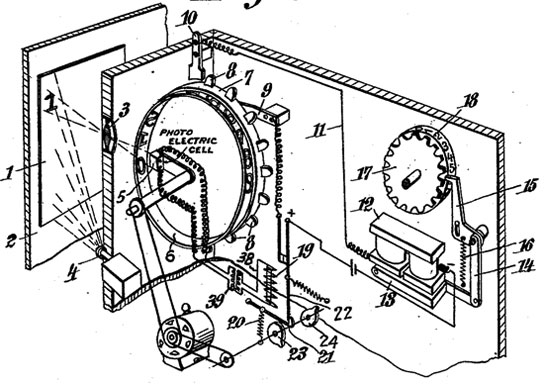
\includegraphics[width=8.5cm]{Tauschek_machine.jpg}
    \caption{La machine à lire de Tauschek. Premier système OCR mécano-électrique. \textcopyright Patent Fetcher}
    \label{fig:tauschek_machine}
\end{wrapfigure}

Concernant l'HTR, on parle de reconnaissance en-ligne (\textit{online}) quand le caractère est reconnu au moment du tracé de la forme ( stylos optiques qui prennent en compte les mouvements) et de reconnaissance hors-ligne (\textit{offline}) quand la reconnaissance du caractère s'effectue sur des caractères déjà tracés sur le papier.\footnote{\cite{eikvil_ocr_1993}}. \\

Concevoir un système suffisamment intelligent capable de reconnaître les écritures humaines et un réel défi. Il est parfois difficile pour une personne de réussir à transcrire dès le premier regard l'écriture de quelqu'un d'autre, on peut notamment penser aux chartes anciennes, ou plus proche de nous, simplement aux ordonnances de médecins.
\newpage
La première invention d'un système de reconnaissance d'écriture remonte à 1929. A cette époque, Gustav Tauschek (1899-1945) crée un premier système basé sur un détecteur photosensible et un faisceau de lumière qui pointe sur un mot (voir Figure \ref{fig:tauschek_machine}). La source lumineuse traverse alors des masques mécaniques (\textit{template}) qui constitue une sorte de bibliothèques de formes de caractères stockés dans une \inquote{mémoire tambour} (également inventé par Tauschek, et ancêtre de nos disques durs actuels). Dès lors, quand la lumière ne passe plus à travers le masque c'est que la forme du caractère contenu dans le mot et le caractère du masque coïncident parfaitement. Le capteur photosensible détecte cette absence de lumière, à ce moment là, un signal est envoyé pour faire tourner le tambour d'impression à la lettre requise, et cette lettre est imprimée sur papier pour l'utilisateur. Cependant, ce principe de masque restait adapté à une quantité de fontes limitées (en cause la mémoire) et bien dessinées. Il ne permettait pas encore de caractériser l'écriture manuscrite basée sur une grande variabilité de formes.\footnote{\cite{ouji_segmentation_2012}}\\

\begin{wrapfigure}[20]{r}{9cm}
    \centering
    \includegraphics[width=7.5cm]{K-NN_schema.png}
    \caption{Illustration simplifiée de la \textit{méthode des k plus proches voisins} (k-NN) \textcopyright L. Terriel, 2020, Diagrams.net}
    \label{fig:k-NN}
\end{wrapfigure}

Durant les années 1960-1965, les premières méthodes HTR basées sur les modèles statistiques et des systèmes de classes contenant plusieurs variantes d'un même caractère émergent. L'image de la lettre et alors comparée à sa classe, et le système estime la distance statistique entre la lettre et ses variantes contenu dans la classe pour déterminer le bon caractère.\\

Parmi les modèles statistiques utilisés la méthode des \textit{k plus proches voisins} (k-NN)\footnote{Voir l'article \cite{noauthor_methode_2020}} : le caractère binarisé est projeté dans un espace vectoriel comme une nouvelle entrée $ x $ qui est comparée à son voisinage de $ k $ (définis comme des échantillons de caractères connus). \\ Le modèle calcule alors la distance minimum entre $ x $ et ses $ k $ voisins pour déterminer $ x $.\\ (Voir la figure \ref{fig:k-NN}) Cependant, cette méthode doit procéder d'un découpage univoque caractère par caractère. Ce qui rend le modèle peut utilisable pour des écritures cursives et rapprochées.\\

En 1974, Raymond Kurzweil, étudiant au MIT (\textit{Massachusetts Institute of Technology}), développe le programme informatique reconnaissant des polices de caractères très différentes, adaptées aux relecteur d'écran pour non-voyants. C'est le premier véritable succès technologique pour la reconnaissance de caractères.\\ 

À partir des années 1980, les modèles mathématiques comme les \textit{modèles de Markov cachés}\footnote{Voir l'article \cite{noauthor_modemarkov_2019}} (\textit{Hidden Markov Model}), sont repris des techniques de reconnaissance de la parole pour être adaptés aux systèmes de reconnaissance des écritures. Les résultats obtenus sont de vrais succès. Combinés à des modèles linguistiques pour reconnaître également la positon des parties dans la phrase, et des méthodes de segmentation avancées, afin d'isoler dans l'image les lignes de texte et les caractères à l'intérieur de celles-ci. ces modèles linguistiques utilisés en \textit{post}-traitement se basent sur des dictionnaires de mots, de syllabes, de \textit{N-grammes} qui réalisent des estimations du nombre d'occurrences de séquences de caractères ou de mots.\\ 

Les années 1990, sont marquées par le retour des technologies de réseaux de neurones. Les systèmes de reconnaissance de caractères s'améliorent nettement en combinaison avec des classifieurs statistiques. Ces méthodes hybrides permettent alors à des entreprises comme IBM, Toshiba, ou Hitachi de créer des chaînes de traitement à grande échelle. Nous pouvons prendre comme exemple le cas du tri postal avec la lecture automatique des codes postaux ou encore les banques avec la détection automatique des zones d'un chèque.
\newpage
\subsection{Modèles de réseaux de neurones profonds appliquées à l'HTR}

\subsubsection{Historique des réseaux de neurones}
La reconnaissance de formes est l'un des enjeu de l'IA à travers la vision par ordinateur. Actuellement, les systèmes HTR les plus performants reposent sur la technologie des réseaux de neurones (Google Tesseract-OCR ou Kraken par exemple). La démocratisation de leurs utilisation via des bibliothèques de code comme \textit{Tensorflow} et \textit{Keras} en langage Python, voient leurs implémentations facilitées. Il s'agit de puissants algorithmes basés sur l'analogie avec la neurobiologie qui peuvent réaliser des tâches et des prédictions dans le contexte pour lequel ils ont été entraînés et cela de manière autonome.\\      

En 1943, Warren McCulloch (1898-1969) un neurologue et Walter Pitts (1923 - 1969) un logicien, proposent dans l'article \inquote{A Logical Calculus of Ideas Immanent in Nervous Activity}\footnote{\cite{mcculloch_logical_1943}} une première représentation du neurone formel. Le neurone y est décrit comme un automate à seuil, dont l'état actif ou non, désigne une valeur logique, vraie ou fausse\footnote{\cite{varela_invitation_1996}, pp.}.\\

Frank Rosenblatt (1928-1971) applique, en 1958, le concept de neurone formel de McCulloch-Pitts en réseau pour simuler le fonctionnement rétinien pour reconnaître des formes. La machine de Rosenblatt ou \textit{perceptron} est la première implémentation de réseaux de neurones muni d'une règle d'apprentissage simple\footnote{\cite{rosenblatt_perceptron_1958}}.\\

Ces approches dites \inquote{connexionistes} vont perdurer jusqu'à atteindre, vers 1970, leurs limites en terme de puissance de calcul pour l'époque. Nous sommes au début de l'architecture Von Neumann pour les ordinateurs et des théories mathématiques.\\

Dans les années 1980, des avancées théoriques majeures améliorent considérablement l'approche des réseaux de neurones comme l'estimation du gradient par rétro-propagation de l'erreur (1989) et analogie des phases d'apprentissages avec les modèles markoviens cachés (1982), et relance le courant \inquote{connexioniste}.\\

Les années 1990 sont alors marquées par une amélioration considérable de la puissance de calcul grâce aux technologies GPU (\textit{Graphics Processing Unit} ou processeurs graphiques) qui permettent d'accélérer les calculs ainsi qu'aux nouveaux algorithmes qui réalisent l'estimation de millions de paramètres du \textit{perceptron} et de créer de nombreuses couches de neurones formels (\textit{layers}) aux fonctions spécifiques. On relève également l'accroissement exponentiel des bases de données qui permettent de tester ces réseaux de neurones avec des données toujours plus nombreuses.

\subsubsection{Du neurone formel aux réseaux de neurones multi-couches : fonctionnement}  

Un neurone formel est à la fois une représentation mathématique et un algorithme informatique basé sur le neurone biologique. On considère généralement un neurone formel qui possède plusieurs entrées $x_1, x_2, ...$ (dendrites) et une sortie $y$ (point de départ de l'axone). L'excitation du synapse est généralement représenté par des coefficients numériques ou poids synaptiques notés $w$. Au cours de l'apprentissage ces coefficients sont ajustés automatiquement. Par exemple, l'algorithme de rétropropagation du gradient, cherche alors à minimiser le gradient d'erreur qui se traduit par l'ajustement des poids synaptiques. On peut également le réaliser manuellement, en fonction des erreurs de sorties. Le neurone simple, comme le \textit{perceptron}, réalise la somme pondérée des entrées : données et poids synaptiques. Le résultat obtenu est passé dans une fonction d'activation ou de transition ($f(n)$), souvent non linéaire. Parmi celle-ci, on retrouve les fonctions sigmoïdes, ReLU, \textit{Softmax} etc. \\ 

On défini généralement un seuil d'activation qui est également un coefficient numérique paramétrable noté le plus souvent $w_0$ ou $\theta$. Si la valeur finale obtenu dépasse ce seuil d'activation, le neurone génère alors une nouvelle sortie $y$. La Figure \ref{fig:neurone_formel} résume ce fonctionnement.
\newpage
\begin{figure}[h]
    \centering
    \centerline{\fbox{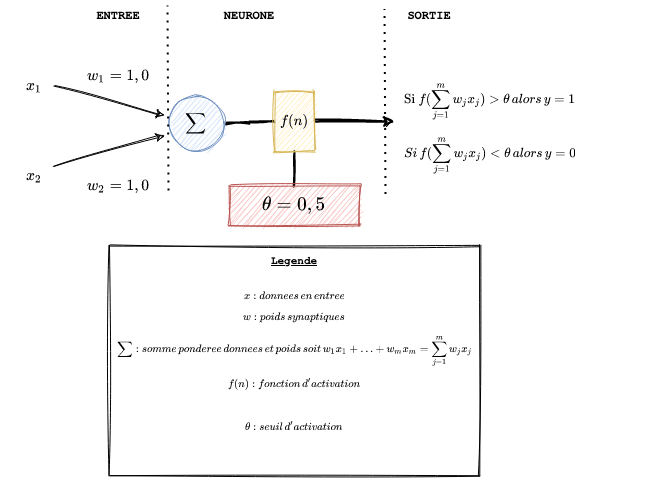
\includegraphics[width=17cm]{neurone_formel.png}}}
    \caption{Illustration simplifiée d'un neurone formel  \textcopyright L. Terriel, 2020, Diagrams.net}
    \label{fig:neurone_formel}
\end{figure}

Le neurone formel est une unité élémentaire dans un réseau de neurones complet. Un réseau de neurones peut donc être représenter sous la forme d'un graphe qui relie plusieurs neurones formels possédant parfois des propriétés ou fonctions d'activation différentes, qui forment une ou plusieurs couches cachées (\textit{Hidden layers}) selon les classes de neurones (réseaux de neurones multi-couches). Ces couches sont généralement définies selon le contexte d'application de ces réseaux comme la reconnaissance de forme, cela procède souvent d'un long travail d'expérimentation même si actuellement des standards se dégagent. Voir la Figure \ref{fig:graph_neurones_artificiels} pour plus de détails.\\

Dans ces réseaux, l'information circule en avant grâce à des algorithmes de propagation (\textit{feed forward propagation}) et des algorithmes de propagation en arrière qui ont des fonctions correctrices (\textit{backward propagation}) des poids synaptiques sur les couches les plus responsables des erreurs. Tout le travail d'ajustement des réseaux pour générer la sortie voulue se situe dans la capacité à corriger les poids synaptiques\footnote{Pour une autre approche des réseaux de neurones on pourra visionner la présentation Mathieu Aubry (École des Ponts ParisTech), \inquote{IA et apprentissage automatique : des outils pour l'analyse et la valorisation du patrimoine}, Journée d'étude \inquote{Intelligence artificielle et institutions patrimoniales} de l'ADEMEC, Bibliothèque nationale de France, 11 décembre 2019, URL : \url{https://www.youtube.com/watch?v=MvaXQ2t2mPs&list=PLayqwLSo_nPW1wHnVw-gJPwMya4gYBPe0&index=2}}.

\newpage
\begin{figure}[h]
    \centering
    \centerline{\fbox{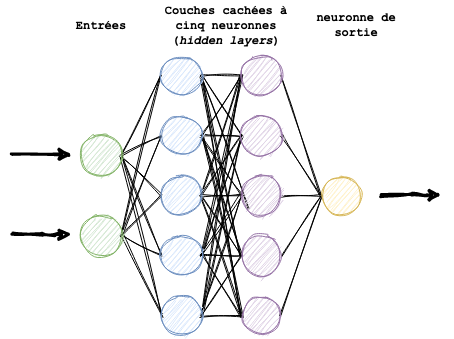
\includegraphics[width=13cm]{graph_neurones_artificiels.png}}}
    \caption{Illustration simplifiée d'un réseau de neurones à deux couches de neurones cachées   \textcopyright L. Terriel, 2020, Diagrams.net}
    \label{fig:graph_neurones_artificiels}
\end{figure}

\subsubsection{Quel réseau de neurones pour l'HTR ?}     

Il existe plusieurs sorte d'architectures pour ces neurones, variant en fonction du contextes d'utilisation, ainsi, dans le cadre de la reconnaissance de formes on utilise des architectures de réseaux de neurones mixtes. Ces dernières utilisent des réseaux de neurones récurrents (RNN ou \textit{Recurrent Neural Network}) chargés de modéliser les séquences de caractères et des réseaux de neurones à convolutions qui quant à eux, permettent d'extraire des caractéristiques (traits, caractères, mots, amas de pixels dans l'image etc.). 

Ces réseaux hybrides sont particulièrement adaptés aux traitements des séquences temporelles comme les phrases qui sont des suites de formes s'enchaînant pour constituer des mots qui demandent de se souvenir des enchaînements de formes précédentes. Parmi les RNN, un type particulier de réseaux de neurones appelé LSTM (\textit{Long short-term memory}) permet de doter le neurone formel de boucles qui lui offre une capacité de mémorisation des enchaînements de formes. Ce réseau hybride est implémenté dans Kraken (Figure \ref{fig:graph_neurones_artificiels}) par le biais de la bibliothèque en langage C++ CLSTM\footnote{CLSTM, est une implémentation des des RNN de type LSTM, voir : \url{https://github.com/tmbdev/clstm}}. 
\begin{figure}[h!]
    \centering
    \centerline{\fbox{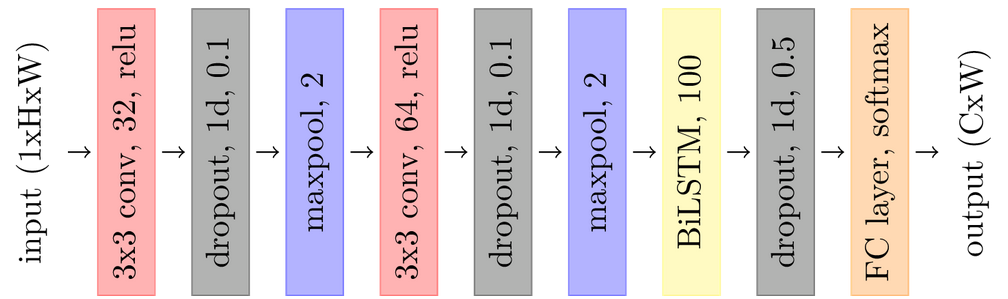
\includegraphics[width=14cm]{reseau_kraken.png}}}
    \caption{Architecture hybride des différentes couches disposant de RNN (BiLSTM) et de neurones à convolution utilisée dans Kraken \textcopyright \cite{kiessling_kraken_2019}}
    \label{fig:graph_neurones_artificiels}
\end{figure}
\newpage
Ces réseaux de neurones sont très gourmands en ressources matérielles. En effet, ils demandent d'effectuer de très nombreux calculs matriciels lors de l'entraînement des modèles, à l'instar des jeux vidéos actuels en haute définition. Dès lors, en l'absence de machines dédiées durant le stage, nous avons bénéficié d'un accès au cluster de calcul de INRIA (RIOC) pour l'entraînement des modèles de transcription et de segmentation sur Kraken. Un cluster de calcul s'apparente à un ordinateur distant (accès sans interface graphique) qui dispose de plusieurs GPU (processeurs graphiques), permettant d'accélérer des traitements informatiques lourds. 

Pour donner un exemple, un ordinateur classique avec un CPU (\textit{central processing unit} ou processeur central) réalise un entraînement en trois à quatre heures, le cluster de calcul réduit à quelques minutes cette charge de travail. L'accès à ce cluster s'effectue via le terminal de l'ordinateur à l'aide de lignes de commandes en BASH permettant une connexion à distance sécurisée (protocole SSH) en sus d'un VPN (\textit{Virtual Private Network} ou réseau privé virtuel).\\ La Figure \ref{fig:epoque_kraken_prompt} donne un exemple d'entraînement sur le cluster.
\newpage
\section{Après l'HTR : extraire, analyser et exploiter les données avec le traitement automatique du langage naturel (TAL)}\label{TAL_repertoire}

On ne pourrait résumer un projet de reconnaissance automatique d'écritures manuscrites à la seule capacité d'un système à produire une bonne transcription, encore faut-il pouvoir exploiter les résultats de l'HTR.\\

La reconnaissance automatique peut-être conçue comme une \textit{pipeline} ou un pont vers l'obtention de données textuelles, possibles grâce aux outils de compréhension du texte, développés dans le domaine du traitement automatique du langage naturel (TAL ou TALN, en anglais \textit{Natural Language Processing} (NLP)).\\

Le TAL est une sous-branche de l'IA, pouvant s'appuyer sur les techniques de ML et DL expliqués plus haut. Ce domaine vise à traiter les langues parlées par les humains. Le TAL couvre donc un large panorama d'applications comme la génération automatique de résumé d'un texte, la traduction d'un document, la recherche d'information, ou encore la \inquote{compréhension} d'un texte (analyse sémantique et syntaxique) pour déterminer le rôle de chaque mot dans une phrase, par exemple. Les tâches techniques du TAL passent par la reconnaissance d'entités nommées, l'extraction de relations, ou encore l'analyse des mots.\\

Dans cette section, nous aborderons, assez succinctement les techniques classiques propres aux TAL. Dans un second volet nous nous attarderons sur les applications de ces techniques dans le projet Lectaurep à destination des publics des archives, des chercheurs ou les archivistes.\\
\newpage
\subsection{Les techniques du TAL}

\textbf{La tokenisation} - C'est le traitement qui permet de découper un texte en phrase, une phrase en mot, ou un mot en lettre. On parle alors de \textit{tokens}. 
\begin{figure}[h]
    \centering
    \centerline{\fbox{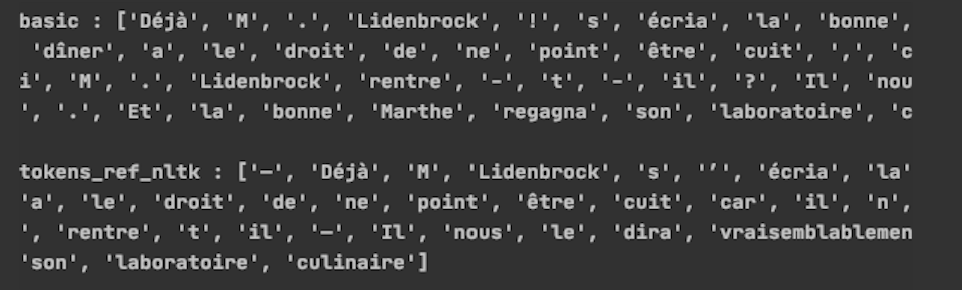
\includegraphics[width=12cm]{TAL_images/tokenisation.png}}}
    \caption{Exemple d'une tokenisation en mots réalisée avec un tokenizer développé à partir des expressions régulières (Regex) et le tokenizer du \textit{package} Python NLTK \textcopyright L. TERRIEL, 2020, \textit{Pycharm}}
    \label{fig:tokenisation}
\end{figure}

\textbf{Enlever les mots les plus fréquents} - Il s'agit généralement de supprimer les mots vides (\textit{stop words}). On considère comme mots vides les occurrences communes qu'il est inutile d'indexer ou d'utiliser car elles peuvent bruiter une recherche ou fausser des résultats. Par exemple, \inquote{le}, \inquote{la}, \inquote{de}, ou \inquote{du} sont des exemples de \textit{stop words}.\\

\textbf{Racinisation} - La racinisation ou désuffixation (\textit{stemming}) consiste à réduire un mot à sa \inquote{racine}. Le but du \textit{stemming} est de regrouper de nombreuses variantes d’un mot comme une seule et même unité. Par exemple, la technique s'appliquant sur \inquote{contrat} et \inquote{contrats} permet de faire ressortir un mot équivalent\footnote{Cette technique est utilisé dans les approches de type sac de mots (\textit{Bag of words}) ou Tf-IdF permettant d'évaluer des occurrences de mots dans un espace vectoriel et qui sont à la base des moteurs de recherche textuels.}.\\

\textbf{Reconnaissance d'entités nommées} - la reconnaissance d'entités nommées (\textit{Named-entity recognition} ou NER) cherche à extraire les entités telles que des personnes, des lieux ou tout autres informations pertinentes pour la compréhension du texte. Certaines applications permettent de visualiser ces entités nommées sous la forme de mots étiquetés sur l'écran (\textit{visualizers}). L'outil Entity-fishing\footnote{\cite{lopez_entity-fishing_nodate}} disponible en ligne offre la possibilité d'extraire les entités nommées d'un texte, de relier ces entités à un référentiel (ici Wikipédia) et de visualiser l'étiquetage des mots. L'étiquetage de ces informations peut être réalisé en JSON (comme dans \textit{Entity-fishing}) ou en XML (Cf. Figure \ref{fig:NER}).

\begin{figure}
    \centering
    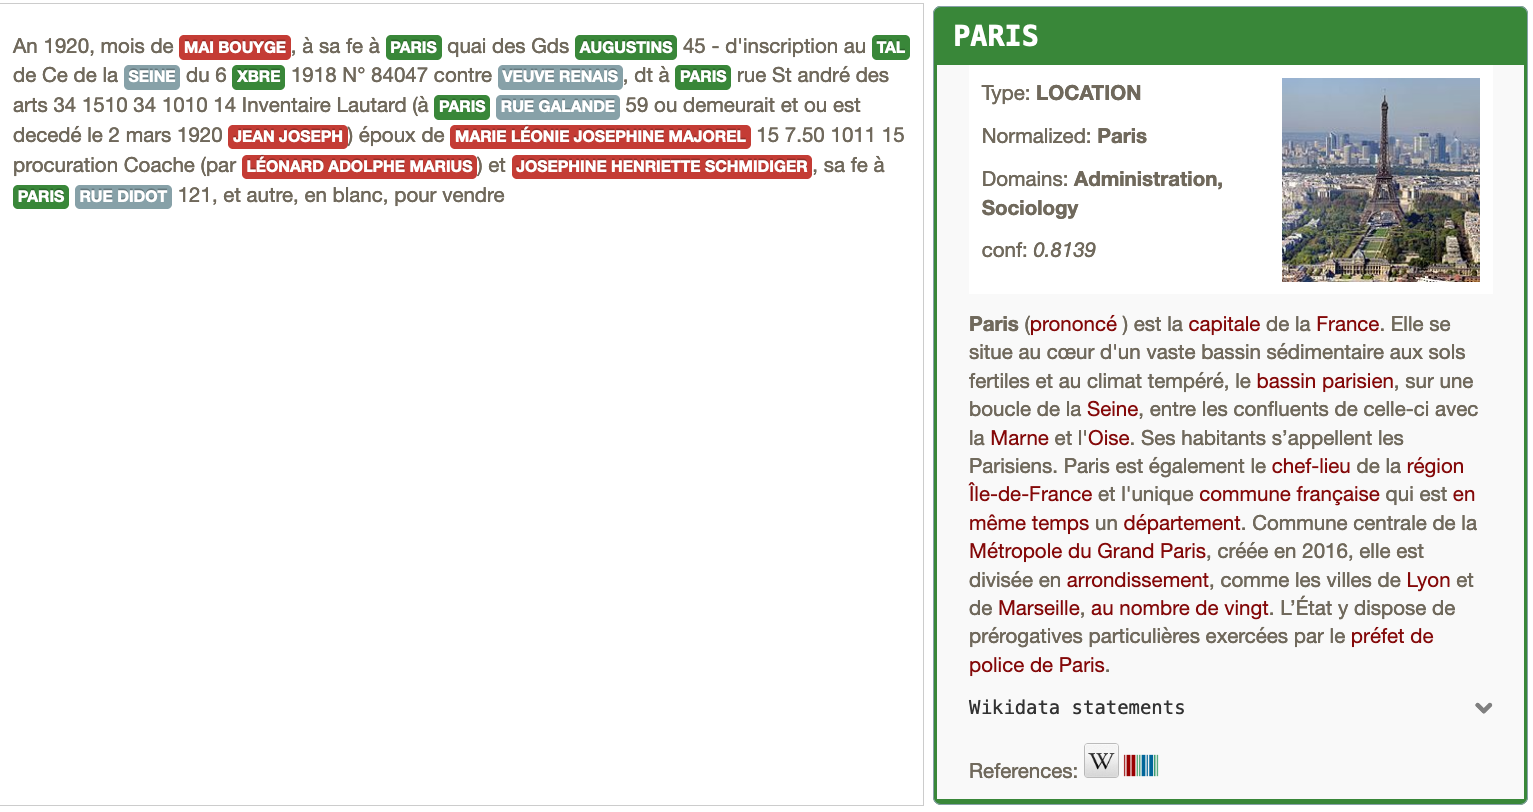
\includegraphics[width=18cm]{TAL_images/exemple_entity-fishing_etiquettes.png}
\end{figure}
\begin{figure}
    \centering
    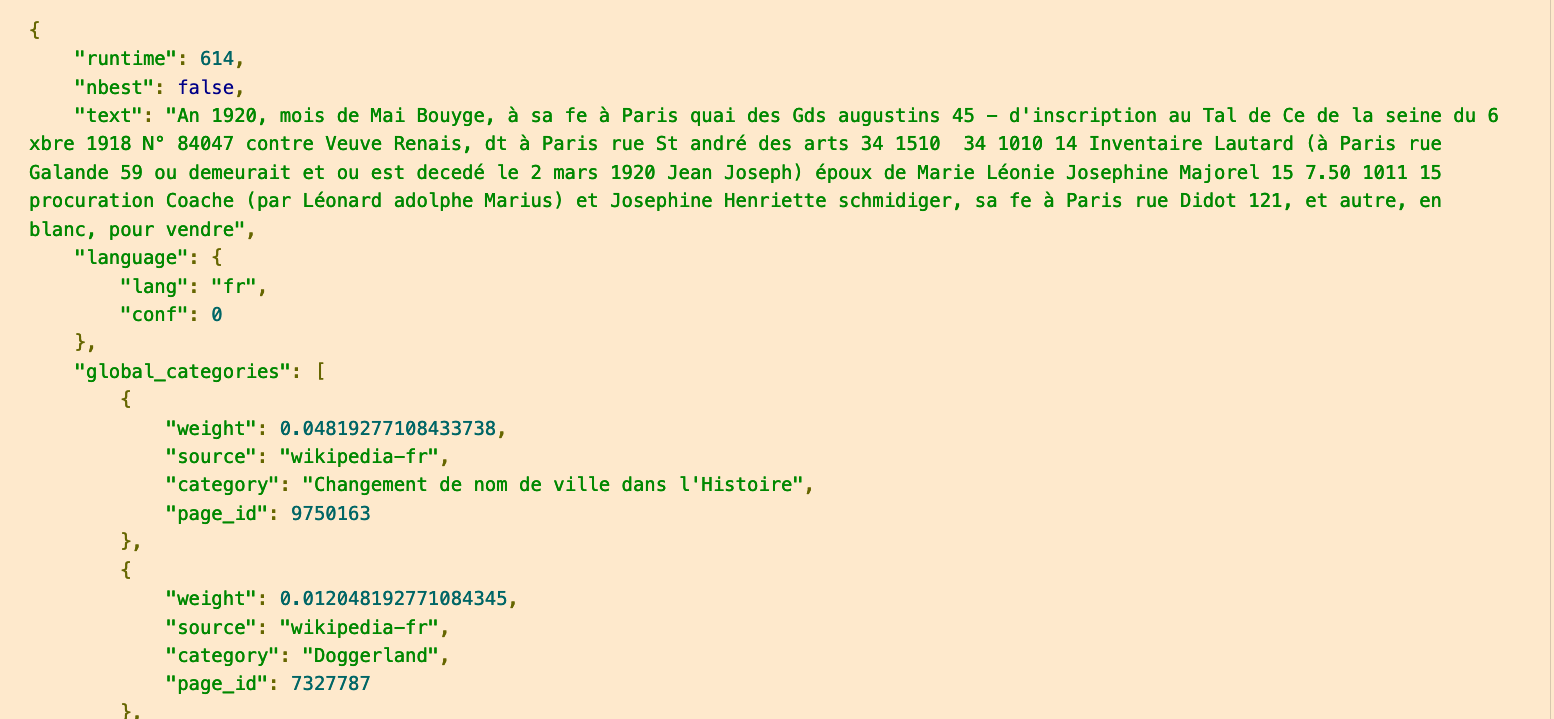
\includegraphics[width=18cm]{TAL_images/entity-fishing_JSON.png}
    \caption{Extrait d'un répertoire du notaire Marotte passé dans l'outil \textit{Entity-fishing} pour l'étiquetage des entités nommées et sa réponse en JSON comprenant le taux de confiance (\textit{weight}) accordé pour chaque candidats du référentiel Wikipédia.  \textcopyright L. TERRIEL, 2020, \textit{Entity-fishing}.}
    \label{fig:NER}
\end{figure}

\newpage
\textbf{L'étiquetage morpho-syntaxique} - L'étiquetage morpho-syntaxique (\textit{Part-of-Speech Tagging} (POS)) consiste à étiqueter la fonction grammaticale de chaque mot dans une phrase. On peut également visualiser ces étiquettes et leurs dépendances (Cf. Figure \ref{fig:NER}).  
\begin{figure}[h]\hspace{-1cm}
    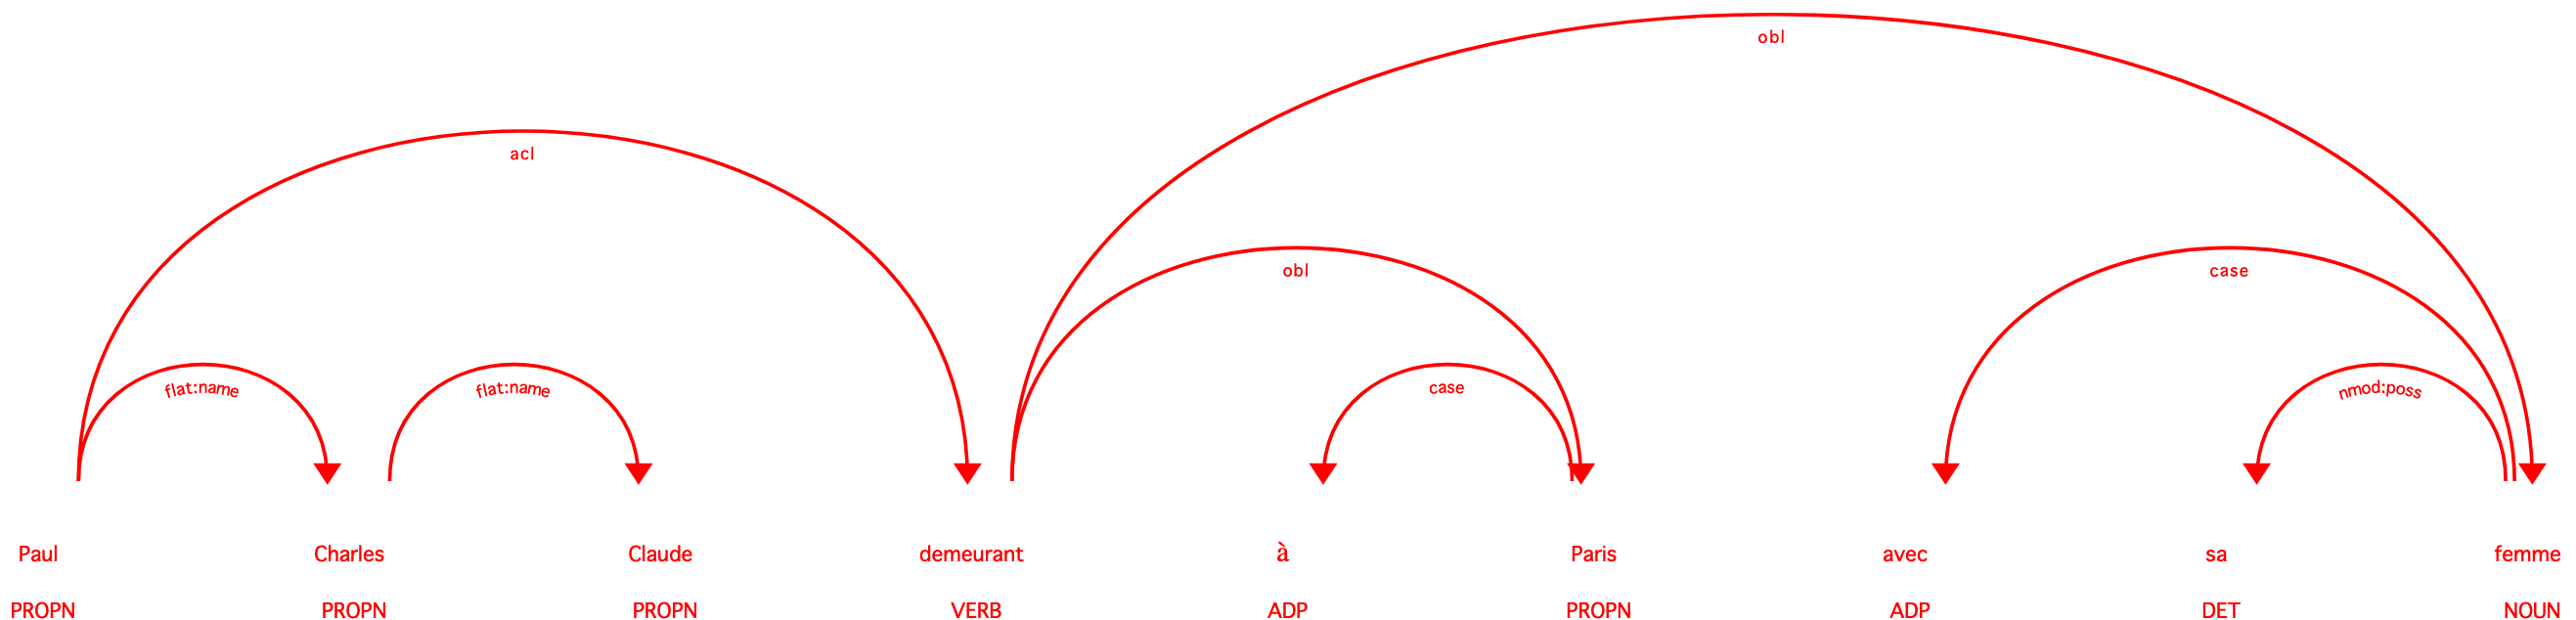
\includegraphics[width=18cm]{TAL_images/POS_example.png}
    \caption{Exemple de POS réalisé sur un document de vérité terrain du répertoire de notaire Marotte. Réalisé avec un script Python (Cf. Annexes, Figure \ref{fig:script_python_POS})  \textcopyright L. TERRIEL, 2020, \textit{Pycharm}.}
    \label{fig:NER}
\end{figure}

\begin{wrapfigure}[15]{r}{8cm}
    \centering
    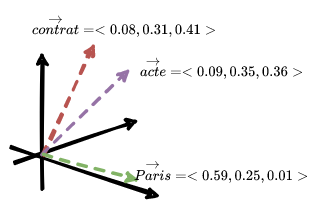
\includegraphics[width=7.5cm]{TAL_images/word_embedding_exemple.png}
    \caption{Exemple simplifié de représentation vectorielle des mots (\textit{Word embedding}). Les mots \inquote{contrat} et \inquote{acte} ont des vecteurs proches (vecteurs colinéaires) tandis que le mot \inquote{Paris} présente un vecteur éloigné par rapport à ses pairs (vecteurs orthogonaux). \textcopyright L. Terriel, 2020, Diagrams.net}
    \label{fig:word_embedding}
\end{wrapfigure}

\textbf{Plongement de mots ou lexical} - Appelé aussi \textit{Word embedding} en anglais, il s'agit d'une méthode qui consiste à représenter les mots sous forme de vecteurs. Cette technique permet notamment de récupérer des valeurs numériques. Ainsi des mots apparaissant dans un même contexte autont des chances d'avoir des vecteurs similaires. On l'utilise notamment pour évaluer la similarité entre des mots ou des phrases grâce aux distances statistiques entre ces vecteurs (par exemple, la distance euclidienne) ou des métriques comme la mesure cosinus (Cf. Partie \ref{partie_3}).\\

\textbf{Modèle \textit{Transformer}} - Plus récents, les modèles \textit{Transformer} sont des modèles de langues entraînés à partir de RNN, comme BERT\footnote{BERT (\textit{Bidirectional Encoder Representations from Transformers}) est un modèle de langage créé par Google, il existe en version multi-language et à été entraîné sur Wikipedia de plus de 104 langues.}, qui sont mises a disposition pour des applications telles que la génération de texte, ou encore la bonne prédiction d'une suite de phrases, et des tâches de question/réponses. BERT dispose de variantes dans d'autres langues, comme CamemBERT qui est un modèle pour la langue française qui a été entraîné par l'équipe d'ALmaNACH avec 130GB de données textuels\footnote{Éric Villemonte de la Clergerie, Yoann Dupont, Louis Martin, Benjamin Muller, Laurent Romary, Benoît Sagot, Djamé Seddah, Pedro Javier Ortiz Suárez, \textbf{BERT}, a Tasty French Language Model, URL : \url{https://arxiv.org/abs/1911.03894}}.

Dans la partie \ref{partie_3}, nous verrons que certaines de ces techniques de TAL nous on été utiles pour l'élaboration de métriques dans notre application d'évaluation des transcriptions Kraken-Benchmark.

\subsection{Les applications et les potentialités du TAL dans Lectaurep}\label{potentialités_TAL}  

Les tâches du TAL décrites plus haut peuvent être mises au service de Lectaurep et plus précisément des résultats des transcriptions obtenu par le modèle HTR.\\

\textbf{Correction des résultats HTR} - Dans un premier cas, les techniques du TAL peuvent permettre d'améliorer les résultats HTR. Ceci peut être réaliser par une combinaison de détection des erreurs de transcriptions et de correcteurs orthographiques en sortie de l'HTR pour corriger les textes de répertoires bruités\footnote{\cite{baranes_vers_2012};  \cite{magallon_detection_2018}}.\\

\textbf{Extraction d'entités nommées et structuration en XML TEI} - L'extraction d'entités nommées dans les répertoires de notaires peut permettre de nombreuses exploitations pour les chercheurs et les publics des archives, les points suivants développe cet aspect. Cependant, comme nous l'avons plus haut cela présuppose de disposer d'un format de données interopérables, comme le JSON ou le XML (comme dans le cas d'\textit{Entity-fishing}). Les \textit{Guidelines P5}\footnote{\cite{tei_consortium_p5_2020}} de la TEI propose un ensemble de balises qui peuvent permettre d'étiqueter les entités nommés repérés dans les répertoires de notaires\footnote{\cite{ruiz_concept-based_2017}} (noms de personnes, dates, biens, types d'actes etc.) mais aussi d'extraire la structure logique des tableaux dans les répertoires\footnote{Cf. Annexes, Figure \ref{fig:tableaux_repertoires}} et la encore de l'exposer dans un modèle TEI. Nous développons ces aspects dans la Partie \ref{partie_2} de ce mémoire.
\newpage
\textbf{Faciliter la recherche dans le répertoire de notaire} - L'extraction d'entités nommés et la structuration en XML TEI peuvent constituer de bons moyens de faciliter l'accès aux corpus d'actes notariés pour les chercheurs et le public des services d'archives. Ils peuvent ainsi formuler plusieurs types de recherche. On distingue généralement : 

\bigskip
\begin{itemize}
    \item La recherche en texte intégral (en texte libre ou plein-texte) : c'est la technique classique d'accès à un mot dans un document éléctronique. Le moteur de recherche examine tous les mots enregistrés dans le document, et essaye de les faire correspondre à le requête de l'utilisateur;\\
    \item La recherche approximative (ou floue ou \textit{fuzzy search}) : il s'agit de trouver un motif (\textit{pattern}) approximatif plutôt qu'une correspondance exacte avec la requête de l'utilisateur composé de sous-chaînes de caractères. Il s'agit donc de proposer des suggestions de recherche ou des corrections orthographiques, plutôt que de répondre directement à la requête de l'utilisateur, qui propose souvent une idée générale plutôt qu'une étiquette technique précise.\\Par exemple, si l'utilisateur effectue une recherche avec le mot-clé \inquote{mariage} le moteur pourra suggérer une formulation plus précise comme \inquote{contrat de mariage}. Cependant, cela demande en amont de calibrer correctement la sensibilité du système afin d'évaluer le niveau d'approximation maximal que l'utilisateur peut proposer lors de sa requête.
    Les algorithmes utilisés pour se type de recherche s'appuient généralement sur les distances d'édition (comme la distance de Levenshtein) et les métriques de similarité que nous rappelons dans la partie \ref{partie_3};\\
    \item La recherche par mots-clés : le principe consiste à extraire certains mots-clés récurrents dans les documents. On peut mentionner la technique de \textit{Keyword spotting}\footnote{Sur les aspects de \textit{Keyword spotting} consulter \cite{bonhomme_defis_2018}, pp.53-55. \\ Le \textit{Keyword spotting} peut également s'appliquer à la recherche de motifs récurrents dans les images (\textit{query by example}). On peut prendre pour exemple de cette recherche les images Isabella di Lenardo (EPFL/INHA/projet Venice Time Machine), \inquote{Chercher dans les grands corpus d'images à travers l'Intelligence Artificielle : défis et résultats}, Journée d'étude \inquote{Intelligence artificielle et institutions patrimoniales} de l'ADEMEC, Bibliothèque nationale de France, 11 décembre 2019, URL : \url{https://www.youtube.com/watch?v=ndT3NLPeQFM&list=PLayqwLSo_nPW1wHnVw-gJPwMya4gYBPe0&index=3})}. Cela permet d'identifier rapidement dans la requête particulièrement longue d'un utilisateur, ces mots-clés et de proposer rapidement les résultats. Cette utilisation des mots-clés peut également constituer une stratégie dans l'élaboration d'une recherche par facettes ou par catégories. 
\end{itemize}
\newpage
\textbf{Liage des entités nommées à d'autres référentiels de données} - Comme nous l'avons déjà cité plusieurs fois, un extracteur d'entités nommés peut-être configuré pour étiqueter mais aussi relier les entités issues des répertoires à des référentiels\footnote{Un \textbf{référentiel} est un moyen de rassembler des connaissances d'un certain type dans des formats structurés (JSON, SQL, ou XML) et normés (TEI, EAD, EAC-CPF, MARC, \textit{Dublin Core} etc.) (taxinomie, ontologie, thésaurus ou vocabulaire controlé).} internes aux Archives nationales, ou externes sous la forme de bases de données présentes sur le \textit{web}. Ainsi un outil comme \textit{Entity-fishing} est paramétrable par le biais de son API ou de son code source pour relier des entités à des référentiels de données du \textit{web} (par défaut, Wikipédia). Cela permettrait à l'utilisateur, dans un premier cas, de visualiser des liens vers d'autres archives pertinentes et insoupçonnées par celui-ci (informations contenues dans les fiches producteurs EAC-CPF ou dans les instruments de recherche en EAD dépendant du système d'information des Archives nationales).\\ 

Dans un second cas, on peut relier ces entités, au travers du \textit{web}, à des bases de données contenant des informations de nature géographiques (GeoNames\footnote{Geonames, URL : \url{https://www.geonames.org/}}), documentaires (data.bnf.fr\footnote{data.bnf.fr, URL : \url{https://data.bnf.fr/}}, Projet Gutenberg\footnote{Projet Gutenberg, URL : \url{https://www.gutenberg.org/browse/languages/fr}}), encyclopédiques (Wikidata\footnote{Wikidata, URL : \url{https://www.wikidata.org/wiki/Wikidata:Main_Page}}), vocabulaire multilingue (Eurovoc\footnote{Eurovoc, URL : \url{https://eur-lex.europa.eu/browse/eurovoc.html?locale=fr}}) etc. C'est une manière de faire entrer le projet dans le cadre des \inquote{données ouvertes liées} (\textit{linked open data}), en rattachant les informations contenues dans les répertoires au \textit{web} sémantique. Cela dans l'optique d'augmenter la pertinence des recherches des utilisateurs de Lectaurep, d'ouvrir la base de connaissances autour des répertoires de notaires et de permettre d'autres axes de lecture de ces sources historiques.\\

\textbf{Une nouvelle approche pour l'histoire notariale} - Le TAL est également une porte d'entrée pour les humanités numériques et ouvre la perspective d'un \inquote{nouveau regard par les historiens}\footnote{\cite{limon-bonnet_innovation_2019}, pp.265}. 
Comme évoqué dans la section \ref{essor_humanités_num}, l'historiographie a soulevé très tôt, l'intérêt de l'usage des archives notariales comme sources pour l'histoire des familles, l'histoire économique et financière ou encore l'histoire administrative, sous l'angle des données quantitatives.  
Dès lors, l'extraction d'informations tels que le prix des actes pratiqués, la taxation de certains actes ou encore le capital des entreprises, autorise, en combinaison avec des outils informatiques de visualisations statistiques, de mener ou de compléter des études sur l'évolution de la fiscalité, de la masse successorale\footnote{La masse successorale est souvent définit comme la part des actifs (ensemble des biens du défunt) dont on déduit un passif (ensemble des dettes).}, et le poids financier des entreprises. Tout cela permet d'évaluer les périodes de creux dans une activité économique. Mais nous ne présentons ici que des exemples des nombreuses approches permises par cette technologie.\\

L'analyse des réseaux (sociaux), approche issue de la sociologie, peut permettre de visualiser les interactions sociales entre des personnes. Cette technique déjà éprouvée en histoire médiévale\footnote{\cite{jegou_potentialites_nodate}} à permis d'augmenter la compréhension l'analyse des réseaux marchands, monastiques, ou d'amitiés. Il en est de même pour les généalogistes pour qui l'étude des lignages, sous la forme de réseaux avec des liens de type orientés (\inquote{être le parent de}) et des liens non-orientés (\inquote{être marié à}), constitue une approche méthodologique valable\footnote{\cite{beauguitte_analyse_2016}, pp.12.}.\\

\begin{figure}[h]
    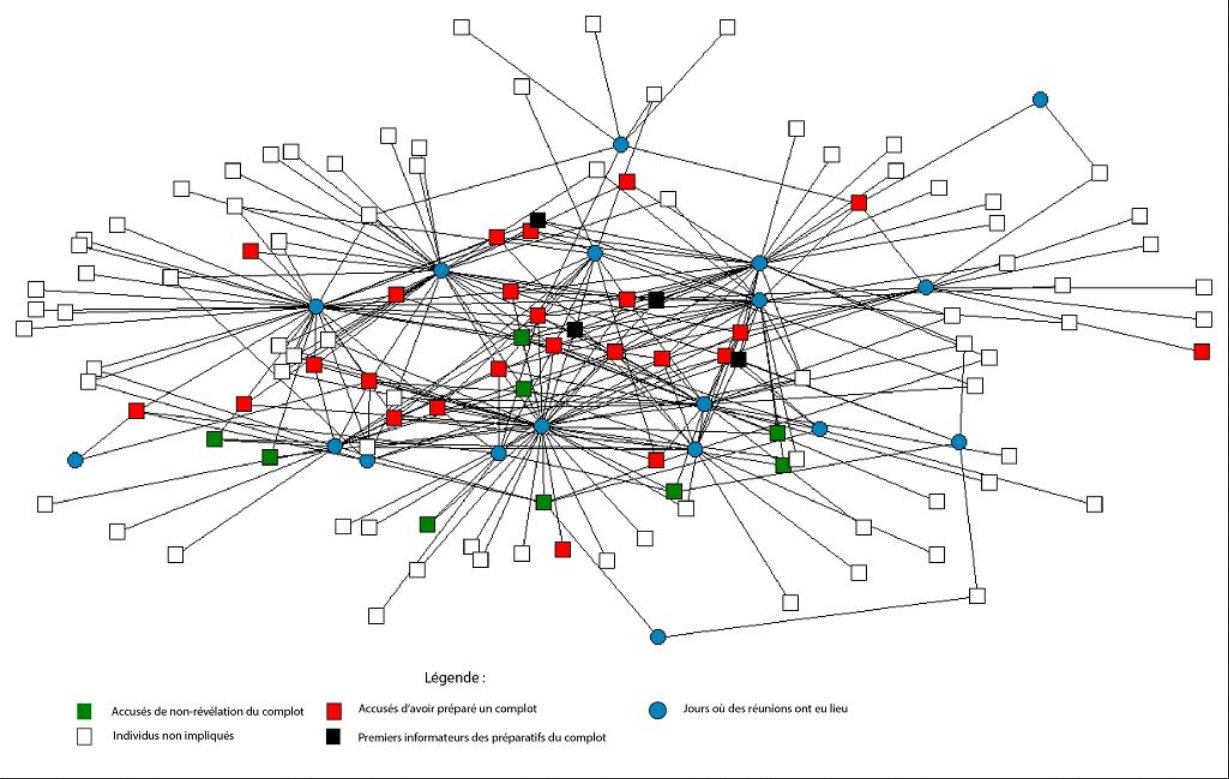
\includegraphics[width=16cm]{TAL_images/exemple_reseaux.png}
    \caption{Un exemple de représentation en réseaux sous la forme d'un graphe entre acteurs du complot (suivant les charges retenues contre eux) et des dates dans le cadre d'une étude du complot 19 août 1820 contre Louis XVIII. \textcopyright\cite{faraut_les_2015}}
    \label{fig:NER}
\end{figure}
\newpage

Cependant, les visualisations en réseaux sont concomitantes de la propreté des données et de leur quantité sélectionnées en amont du projet. Un trop grand nombre de données peut faire croître le nombre de relations ce qui peut rapidement rendre illisible le graphe de données\footnote{\cite{beauguitte_analyse_2016}, pp.}.\\

Ces visualisations ne se limitent pas aux relations entre personnes, mais s'intéressent également aux données géographiques. L'usage d'outils développés dans le cadre des humanités numériques comme, par exemple, Palladio\footnote{Standford University, \textit{Palladio}, URL :  \url{https://hdlab.stanford.edu/palladio/}}, développé par l'Université de Standford, permettent alors de cartographier ou de visualiser de vastes ensembles de données géolocalisées.\\

Pour Lectaurep, les outils de visualisations en réseaux constitue une plus-value pour l'évaluation de la répartition topographique et géographique de la clientèle, le rayonnement de l'activité d'un notaire sur des cartes de l'époque.\\

Analyses statistiques et visualisations en réseaux augmentent la compréhension de l'activité notariale à partir des informations contenues dans les répertoires, une structure en TEI peut également favoriser les études paléographiques des écritures XIX$^{e}$ siècle. La constitution d'éditions électroniques des répertoires de notaires serait augmentée par le repérage de la structure logique du répertoire, des aspects matériels (qualité du papier) et d'éléments caractéristiques de certaines écritures XIX$^{e}$ siècle\footnote{Cf. Figure \ref{fig:ecritures_XIX}}. Une structuration en XML TEI permet des transformations vers le HTML, principal langage du \textit{web}, pour proposer des visualisations sur la base de fac-similés interactifs à l'image des \inquote{dossiers documentaires} proposés par la base \textit{Theleme} de l'École nationale des chartes\footnote{Theleme/École nationale des chartes, \inquote{Dossiers documentaires}, URL : \url{http://theleme.enc.sorbonne.fr/dossiers/index.php}}. Ces aspects sont développés dans la partie suivante.
\newpage
\thispagestyle{empty}

